\newpage
\section{Sidebands}
\label{sec:sidebands}

To validate the modelling of neutrino interactions in MicroBooNE and predicted sources of background, several sidebands are employed. These consist of the events selected by the muon neutrino constraint selection, events containing two or more reconstructed showers to study the $\pi^0$ induced backgrounds and shower energy estimation, and near/far sidebands created with combinations of higher energy/lower BDT scoring events. The selections used to obtain the near/far sidebands will be detailed in Section~\ref{sec:NearAndFarSideband}.

These comparisons are not only to ensure the overall data/simulation agreement, but stability in the behavior of the data and simulation across the different runs. To this end, we will study data to simulation comparisons from runs 1-3, runs 4-5, and runs 1-5, the first example of which is shown in Figure~\ref{fig:NuMuSideband}. 

\subsection{$\nu_{\mu}$ Events}
\label{sec:NuMuSideband}

This sideband is obtained by applying the full muon neutrino event selection described in Section~\ref{sec:EventSelections}. This sideband is used to constrain the prediction in the signal region. Predictions are compared to data from the different epochs in Figure~\ref{fig:NuMuSideband}, for the reconstructed muon energy, muon candidate direction, and reconstructed neutrino energy, showing agreement within uncertainties in all three variables, and good stability across the runs.

\begin{figure}[H]
    \centering
    \begin{subfigure}{0.33\linewidth}
        \captionsetup{width=0.7\linewidth}
        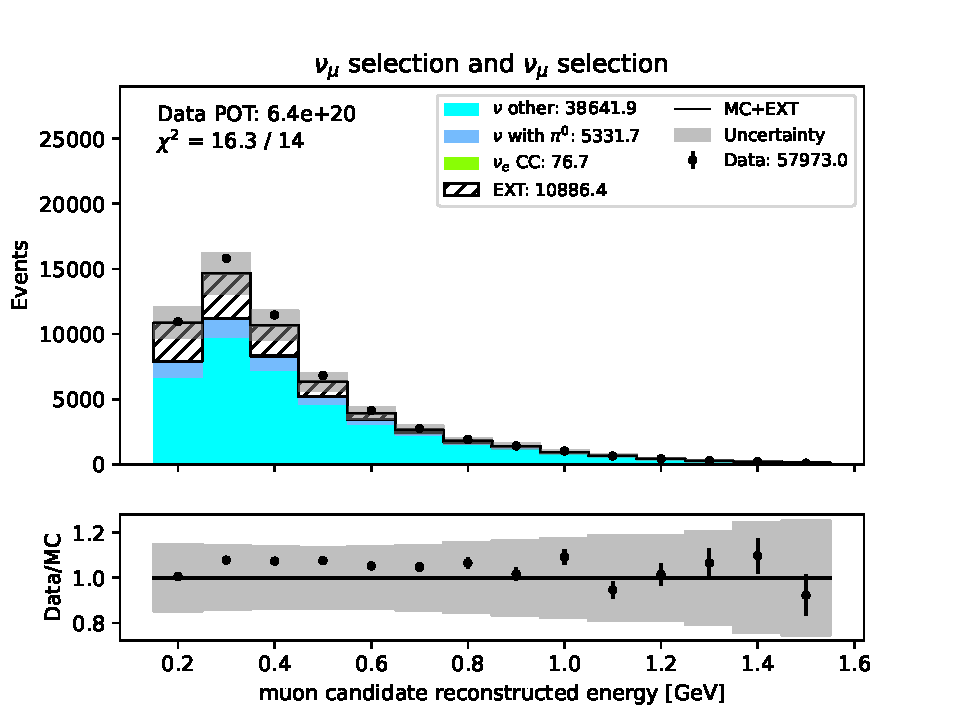
\includegraphics[width=\linewidth]{technote/Sidebands/Figures/NuMuSideband/muon_sideband_muon_energy_run123_NUMU_NUMU.pdf}
        \caption{Muon reconstructed energy, runs 1-3.}
    \end{subfigure}%
    \begin{subfigure}{0.33\linewidth}
        \captionsetup{width=0.6\linewidth}
        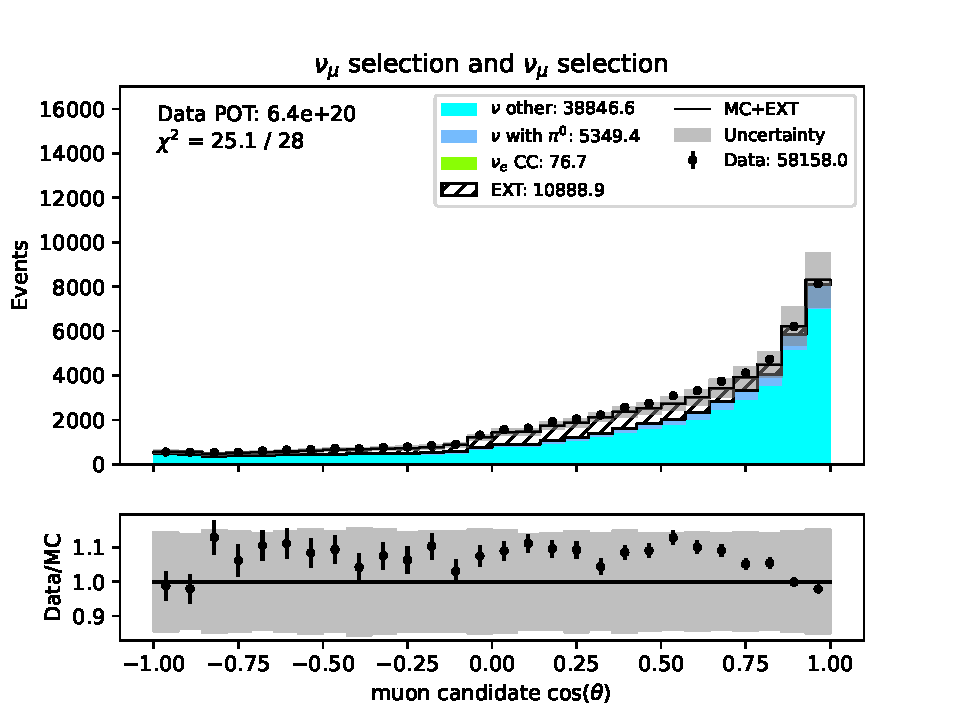
\includegraphics[width=\linewidth]{technote/Sidebands/Figures/NuMuSideband/muon_sideband_muon_theta_run123_NUMU_NUMU.pdf}
        \caption{Muon candidate direction, runs 1-3.}
    \end{subfigure}%
    \begin{subfigure}{0.33\linewidth}
        \captionsetup{width=0.7\linewidth}
        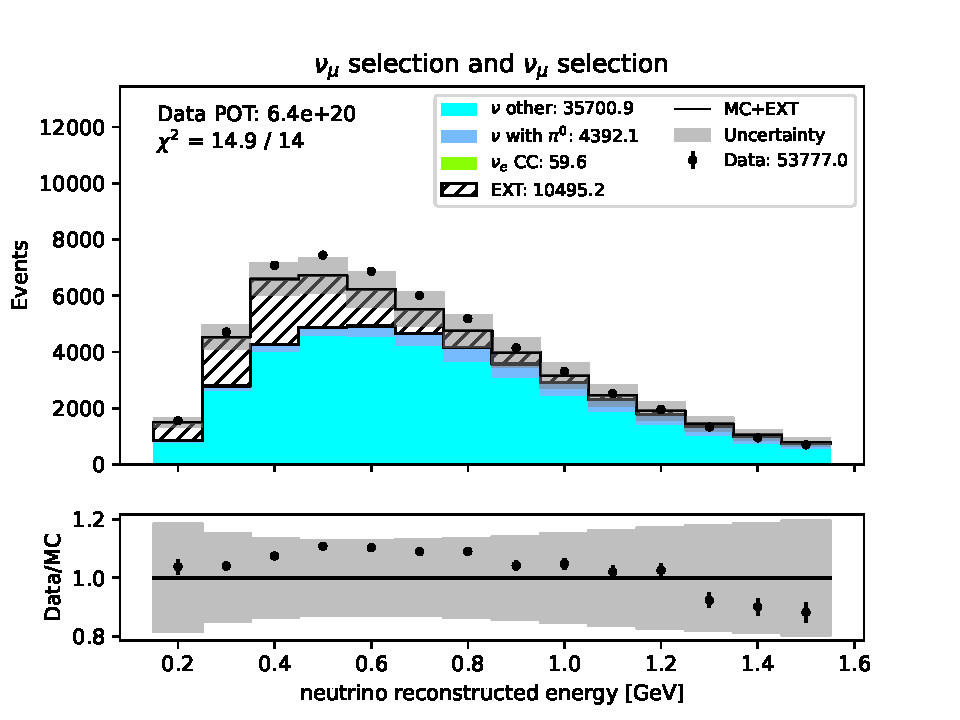
\includegraphics[width=\linewidth]{technote/Sidebands/Figures/NuMuSideband/muon_sideband_neutrino_energy_run123_NUMU_NUMU.pdf}
        \caption{Reconstructed neutrino energy, runs 1-3.}
    \end{subfigure}
    \begin{subfigure}{0.33\linewidth}
        \captionsetup{width=0.7\linewidth}
        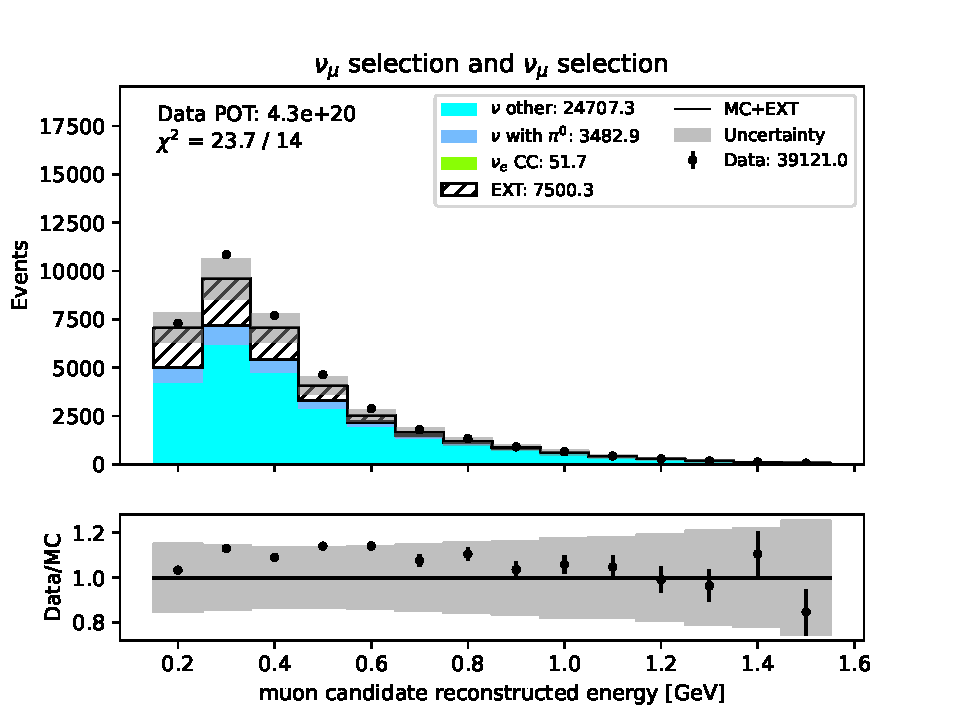
\includegraphics[width=\linewidth]{technote/Sidebands/Figures/NuMuSideband/muon_sideband_muon_energy_run4b4c4d5_NUMU_NUMU.pdf}
        \caption{Muon reconstructed energy, runs 4-5.}
    \end{subfigure}%
    \begin{subfigure}{0.33\linewidth}
        \captionsetup{width=0.6\linewidth}
        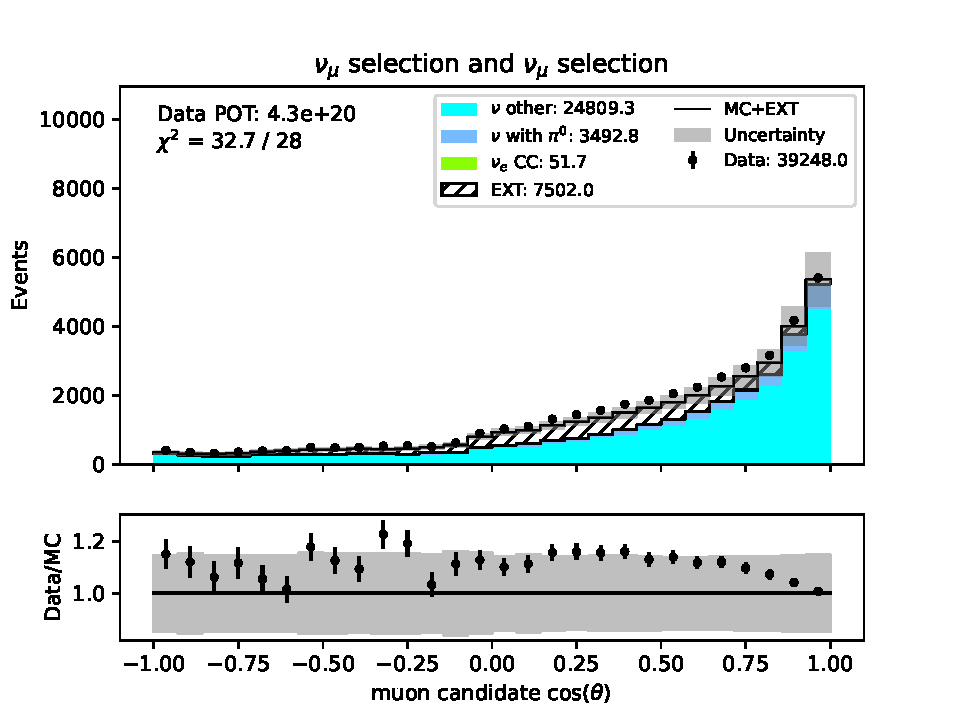
\includegraphics[width=\linewidth]{technote/Sidebands/Figures/NuMuSideband/muon_sideband_muon_theta_run4b4c4d5_NUMU_NUMU.pdf}
        \caption{Muon candidate direction, runs 4-5.}
    \end{subfigure}%
    \begin{subfigure}{0.33\linewidth}
        \captionsetup{width=0.7\linewidth}
        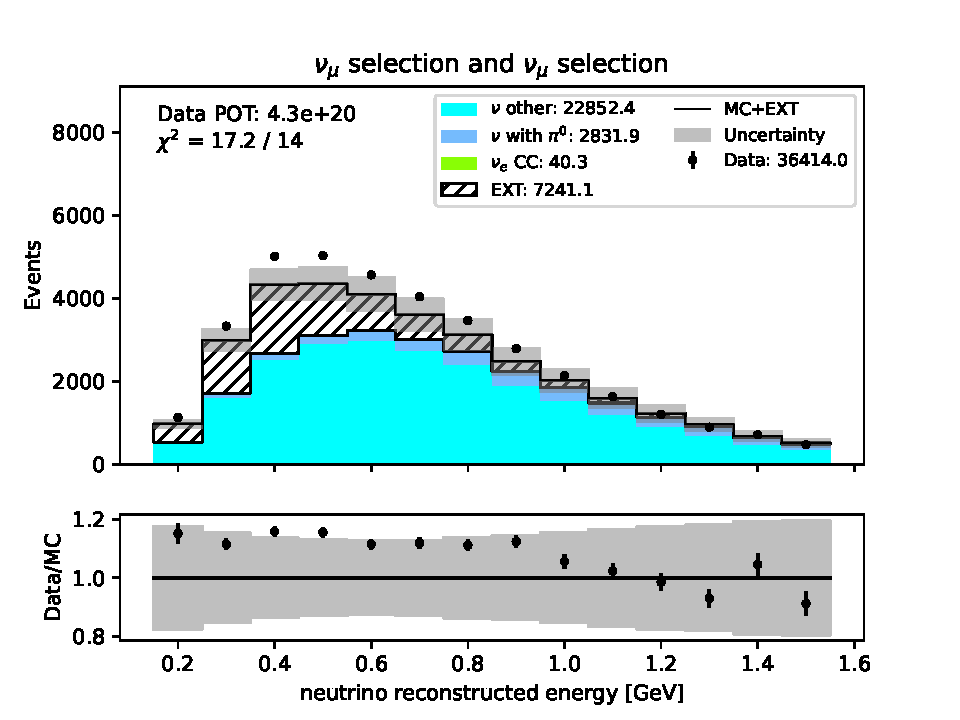
\includegraphics[width=\linewidth]{technote/Sidebands/Figures/NuMuSideband/muon_sideband_neutrino_energy_run4b4c4d5_NUMU_NUMU.pdf}
        \caption{Reconstructed neutrino energy, runs 4-5.}
    \end{subfigure}    
    \begin{subfigure}{0.33\linewidth}
        \captionsetup{width=0.7\linewidth}
        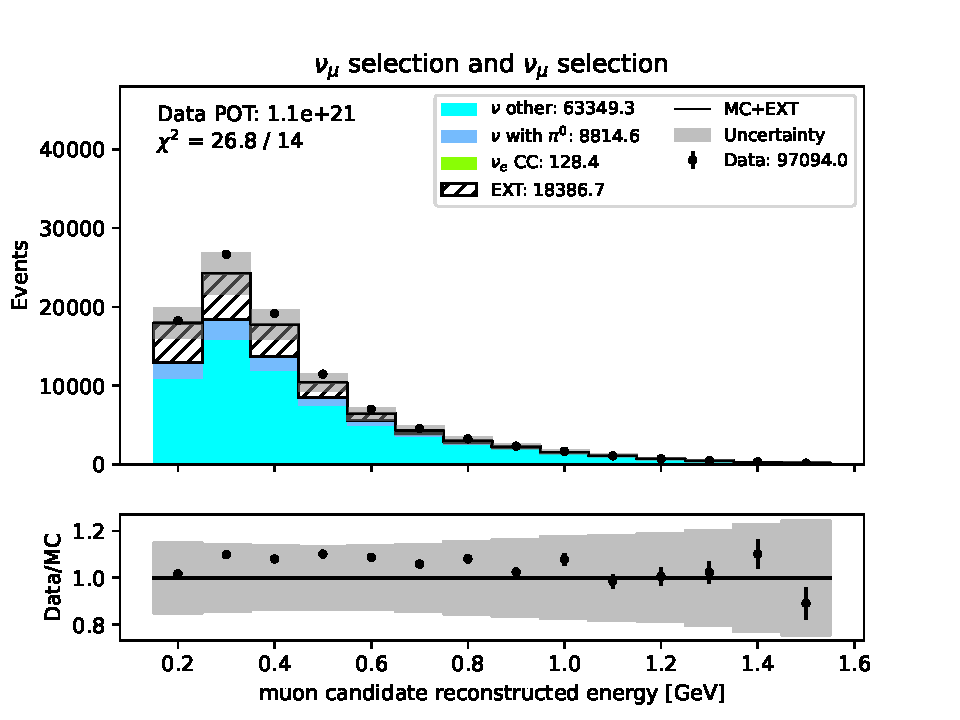
\includegraphics[width=\linewidth]{technote/Sidebands/Figures/NuMuSideband/muon_sideband_muon_energy_run1234b4c4d5_NUMU_NUMU.pdf}
        \caption{Muon reconstructed energy, runs 1-5.}
    \end{subfigure}%
    \begin{subfigure}{0.33\linewidth}
        \captionsetup{width=0.6\linewidth}
        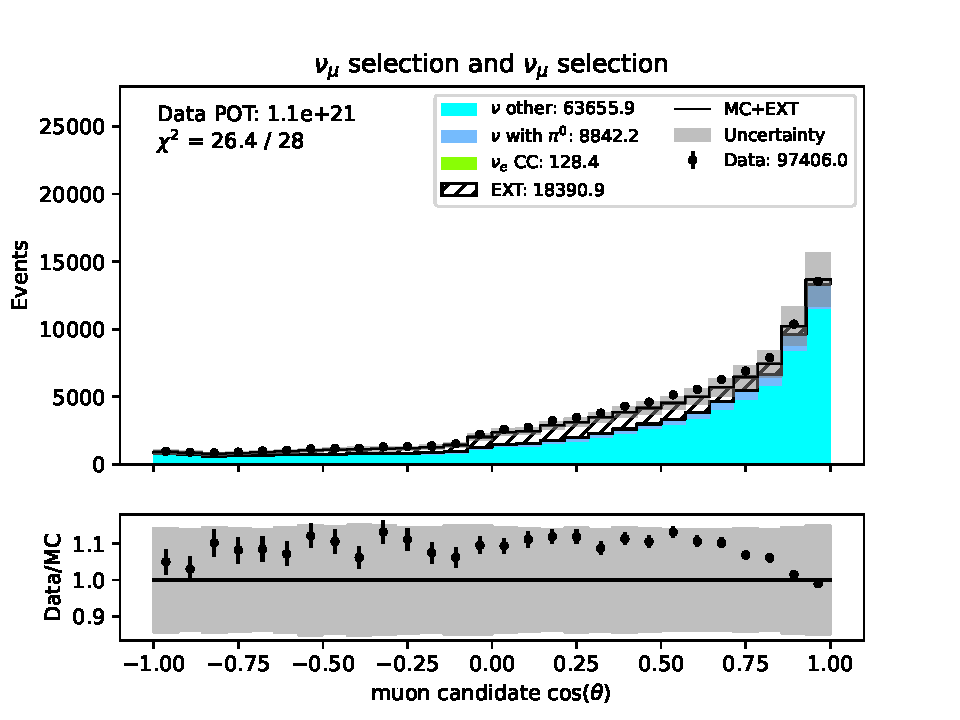
\includegraphics[width=\linewidth]{technote/Sidebands/Figures/NuMuSideband/muon_sideband_muon_theta_run1234b4c4d5_NUMU_NUMU.pdf}
        \caption{Muon candidate direction, runs 1-5.}
    \end{subfigure}%
    \begin{subfigure}{0.33\linewidth}
        \captionsetup{width=0.7\linewidth}
        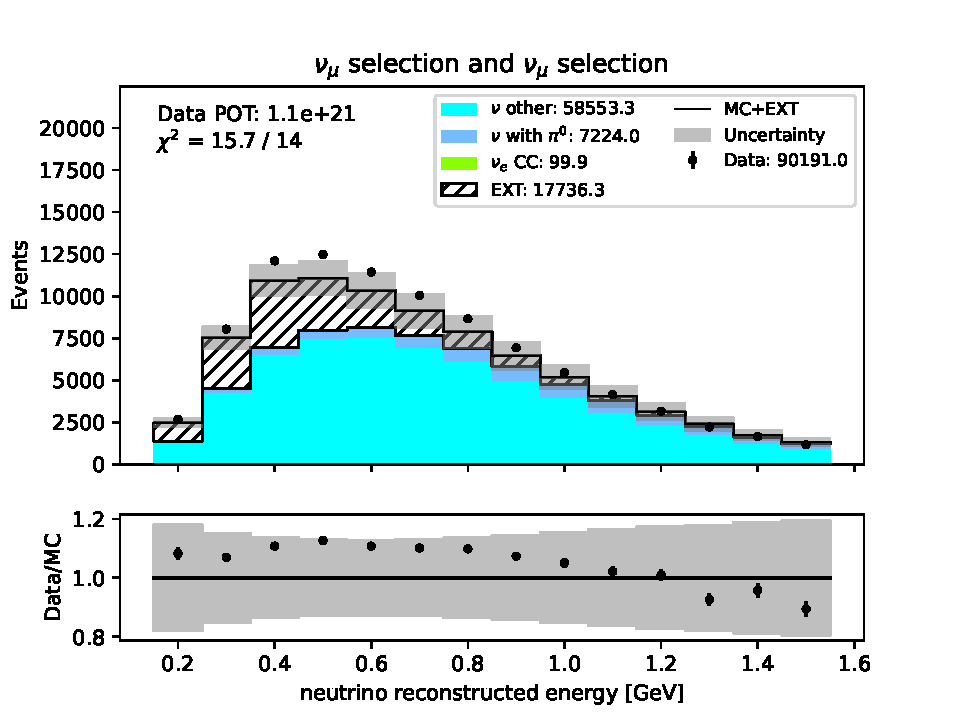
\includegraphics[width=\linewidth]{technote/Sidebands/Figures/NuMuSideband/muon_sideband_neutrino_energy_run1234b4c4d5_NUMU_NUMU.pdf}
        \caption{Reconstructed neutrino energy, runs 1-5.}
    \end{subfigure}
    \caption{Data and MC simulation comparisons after applying the muon sideband selection from Table~\ref{appendix:NuMuSelection}.}
    \label{fig:NuMuSideband}
\end{figure}
\subsection{Two Shower Sideband}
\label{sec:TwoShowerSideband}

This sideband is chosen to better understand the detector response to electromagnetic showers and the background induced by neutral pion production. No pion background scaling is applied to the following plots, and there is an overprediction of this background shown across all runs, which was also observed in the previous analysis. No $\pi^0$ tune was used in the final version of the run 1-3 analysis, so we are not using one here. 

\begin{figure}[H]
    \centering
    \begin{subfigure}{0.33\linewidth}
        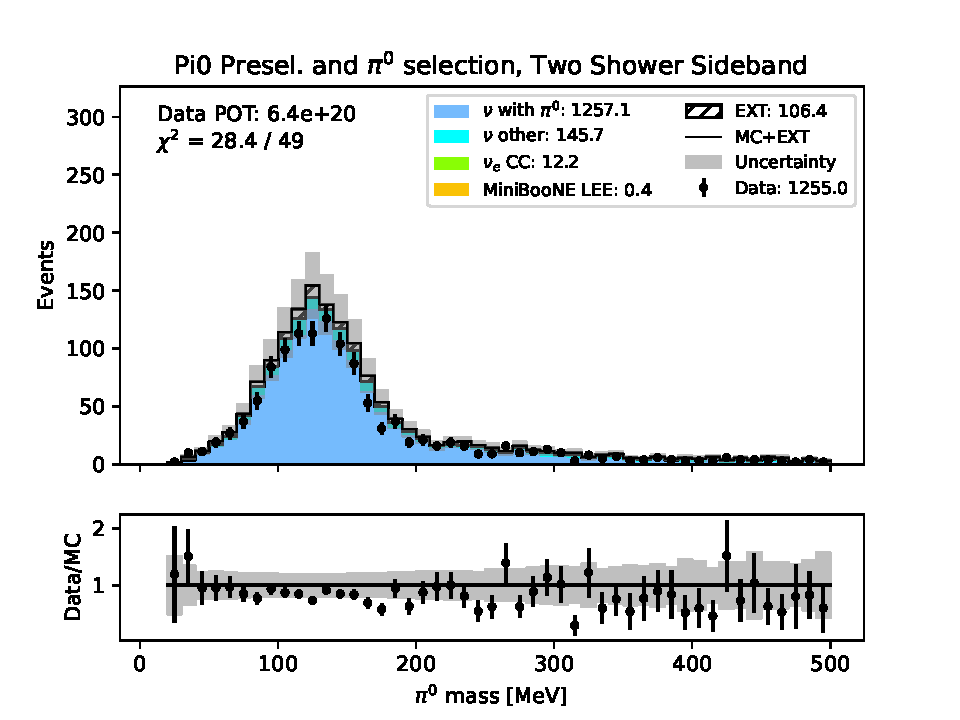
\includegraphics[width=\linewidth]{technote/Sidebands/Figures/TwoShowerSideband/two_shr_sideband_pi0_mass_Y_corr_run123_PI0_PI0.pdf}
        \caption{Reconstructed $\pi^0$ mass, runs 1-3.}
    \end{subfigure}%
    \begin{subfigure}{0.33\linewidth}
        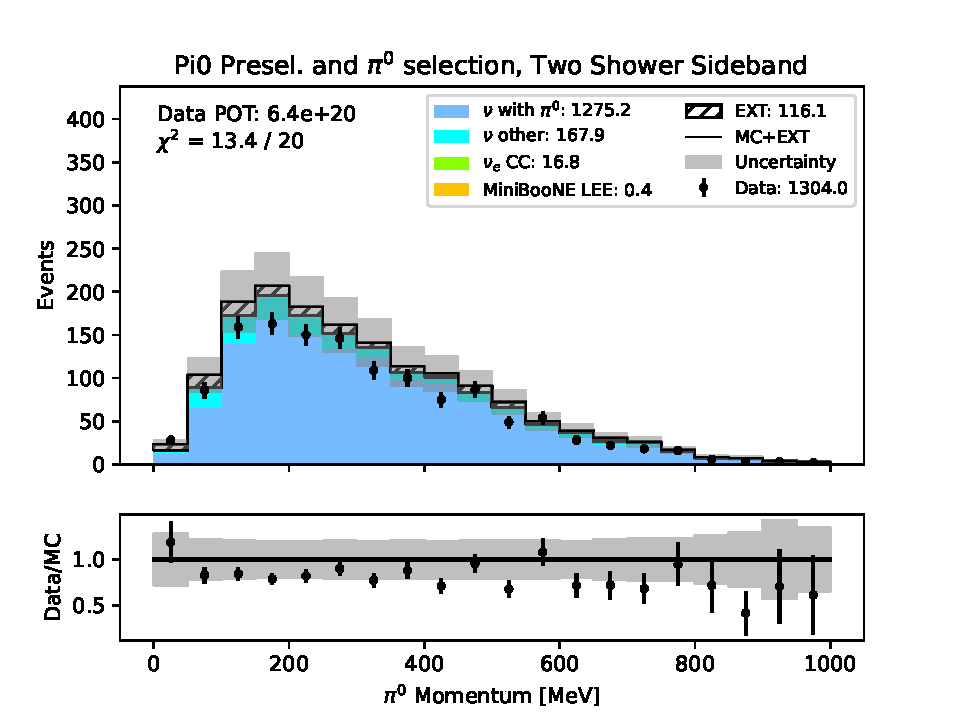
\includegraphics[width=\linewidth]{technote/Sidebands/Figures/TwoShowerSideband/two_shr_sideband_pi0momentum_run123_PI0_PI0.pdf}
        \caption{Reconstructed $\pi^0$ momentum, runs 1-3.}
    \end{subfigure}%
    \begin{subfigure}{0.33\linewidth}
        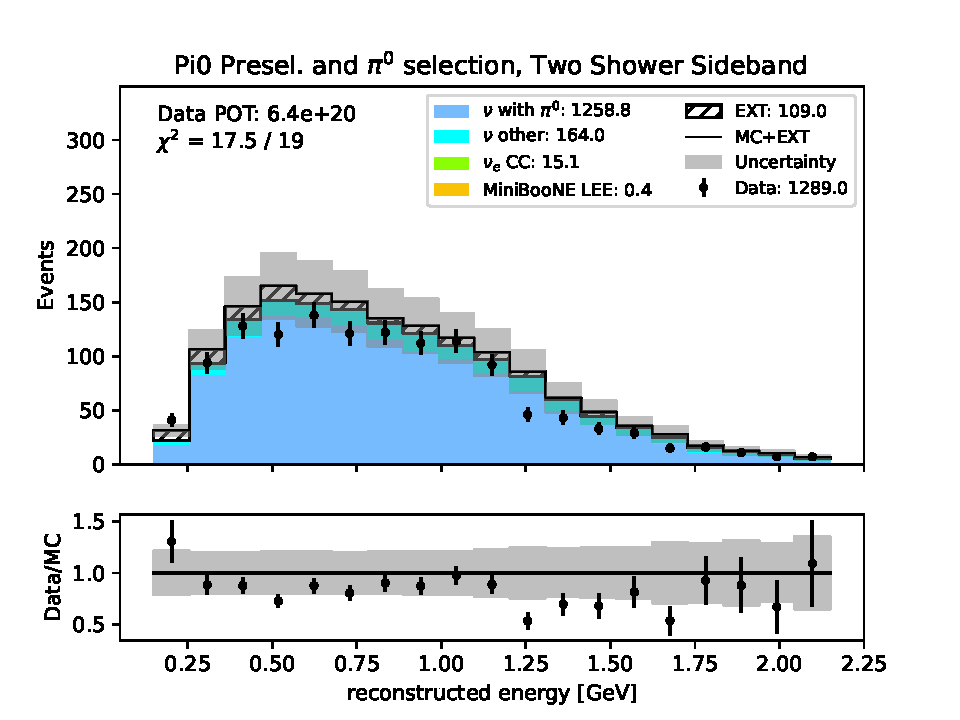
\includegraphics[width=\linewidth]{technote/Sidebands/Figures/TwoShowerSideband/two_shr_sideband_reco_e_run123_PI0_PI0.pdf}
        \caption{Reconstructed neutrino energy, runs 1-3.}
    \end{subfigure}
    \begin{subfigure}{0.33\linewidth}
        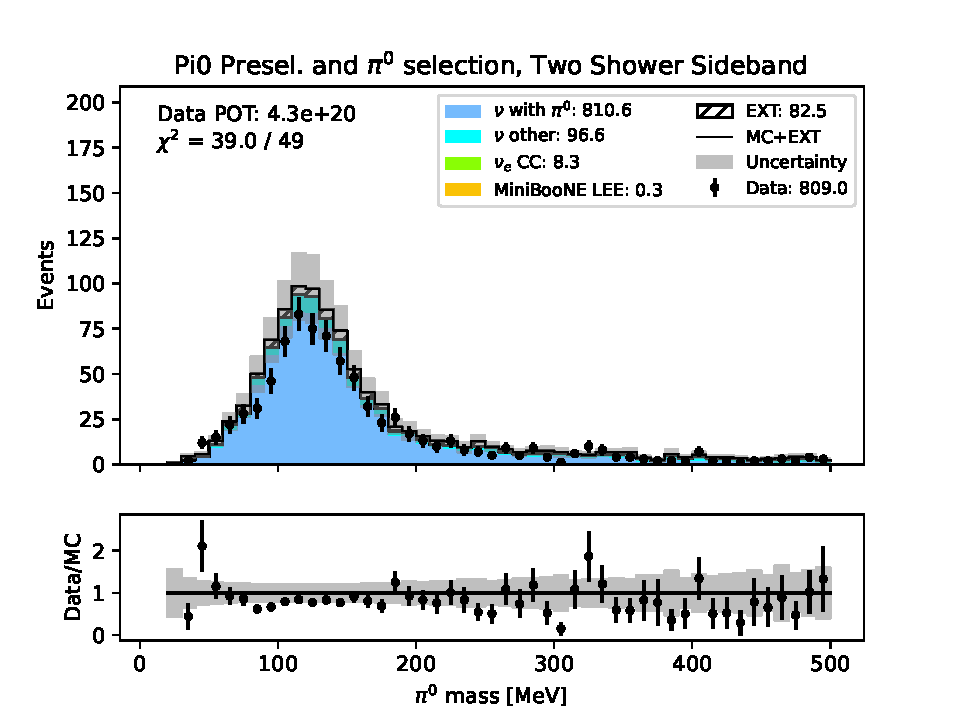
\includegraphics[width=\linewidth]{technote/Sidebands/Figures/TwoShowerSideband/two_shr_sideband_pi0_mass_Y_corr_run4b4c4d5_PI0_PI0.pdf}
        \caption{Reconstructed $\pi^0$ mass, runs 4-5.}
    \end{subfigure}%
    \begin{subfigure}{0.33\linewidth}
        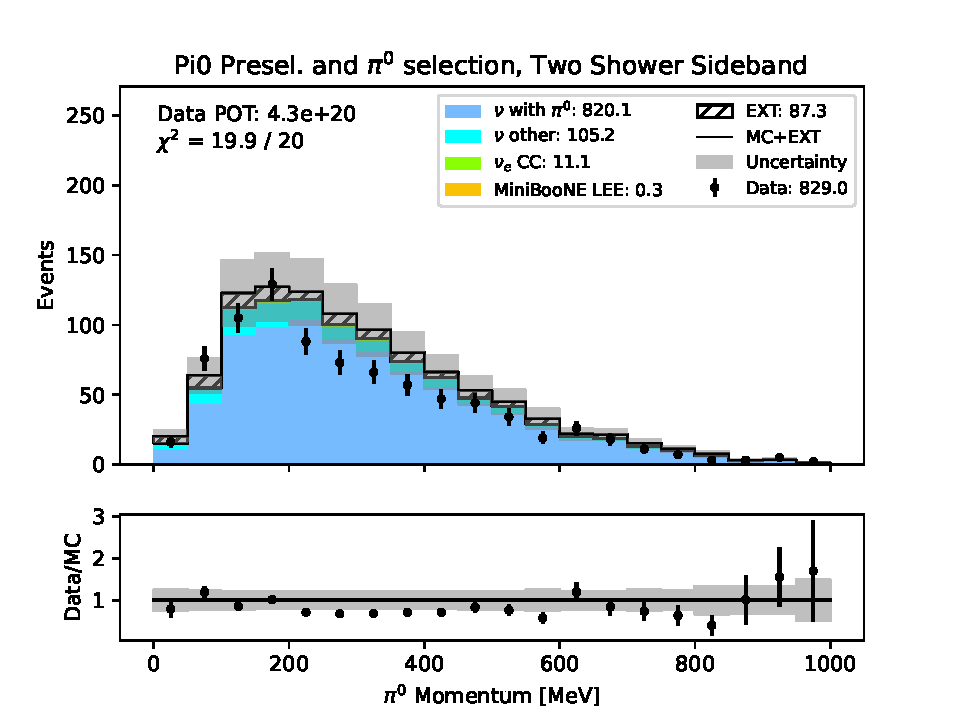
\includegraphics[width=\linewidth]{technote/Sidebands/Figures/TwoShowerSideband/two_shr_sideband_pi0momentum_run4b4c4d5_PI0_PI0.pdf}
        \caption{Reconstructed $\pi^0$ momentum, runs 4-5.}
    \end{subfigure}%
    \begin{subfigure}{0.33\linewidth}
        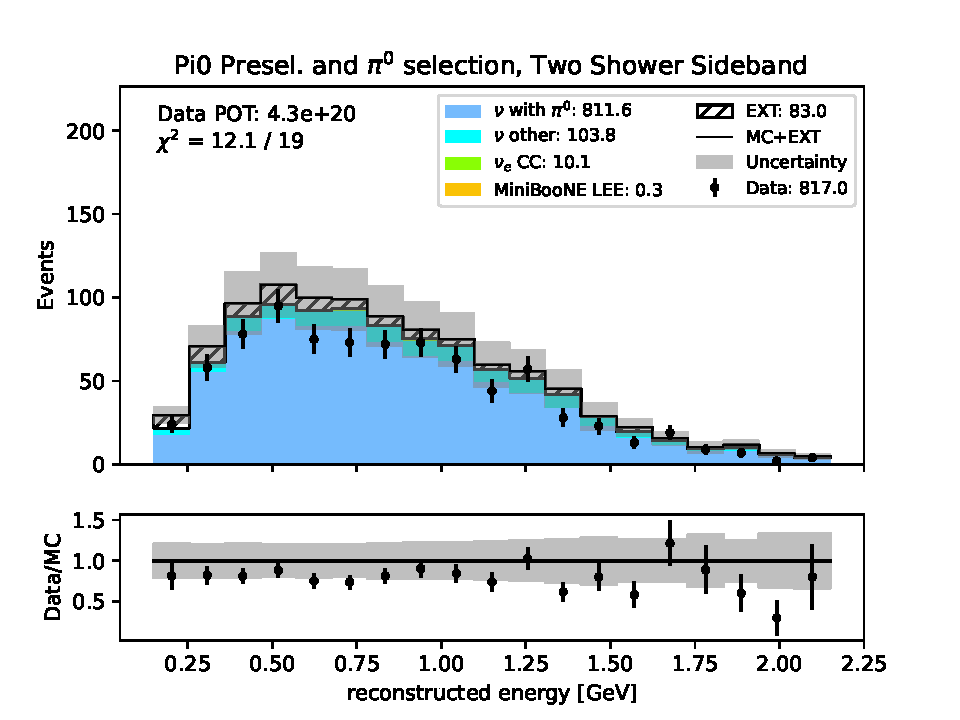
\includegraphics[width=\linewidth]{technote/Sidebands/Figures/TwoShowerSideband/two_shr_sideband_reco_e_run4b4c4d5_PI0_PI0.pdf}
        \caption{Reconstructed neutrino energy, runs 4-5.}
    \end{subfigure}
    \begin{subfigure}{0.33\linewidth}
        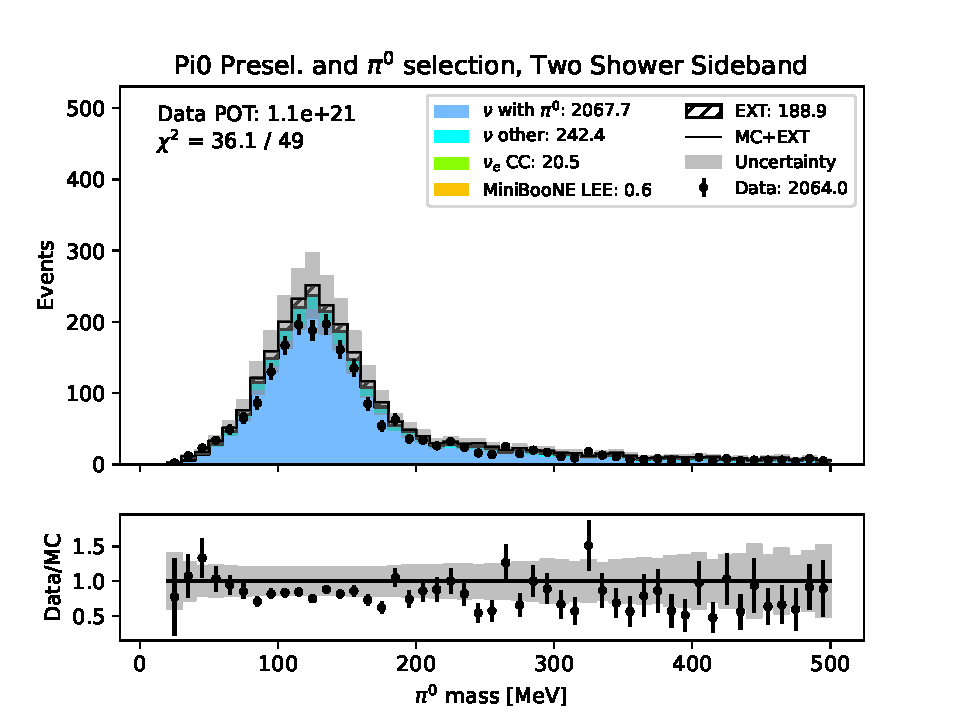
\includegraphics[width=\linewidth]{technote/Sidebands/Figures/TwoShowerSideband/two_shr_sideband_pi0_mass_Y_corr_run1234b4c4d5_PI0_PI0.pdf}
        \caption{Reconstructed $\pi^0$ mass, runs 1-5.}
    \end{subfigure}%
    \begin{subfigure}{0.33\linewidth}
        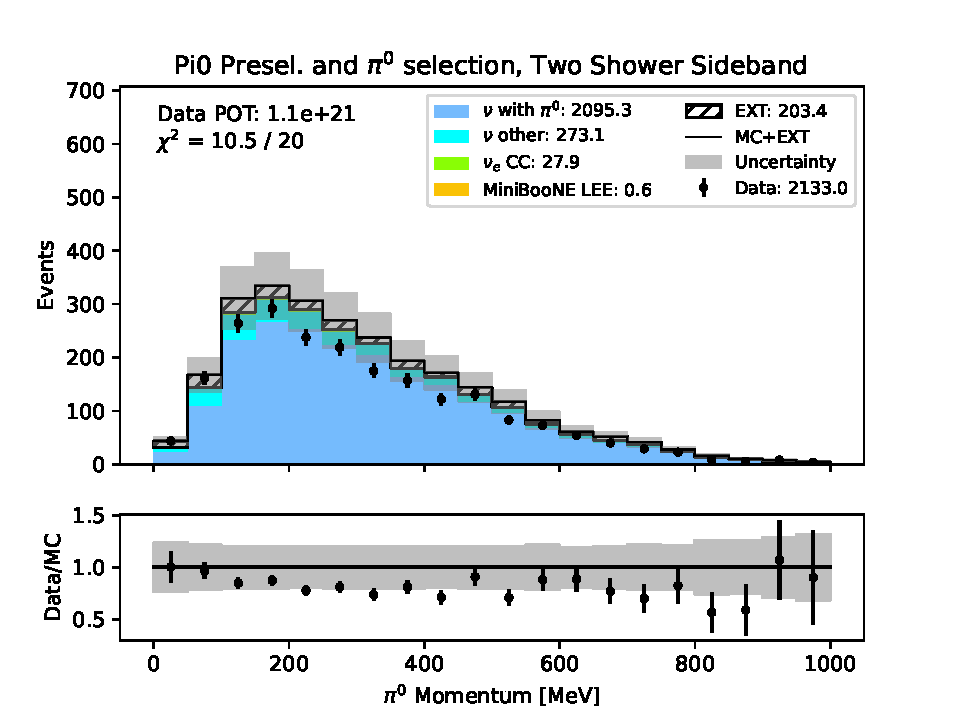
\includegraphics[width=\linewidth]{technote/Sidebands/Figures/TwoShowerSideband/two_shr_sideband_pi0momentum_run1234b4c4d5_PI0_PI0.pdf}
        \caption{Reconstructed $\pi^0$ momentum, runs 1-5.}
    \end{subfigure}%
    \begin{subfigure}{0.33\linewidth}
        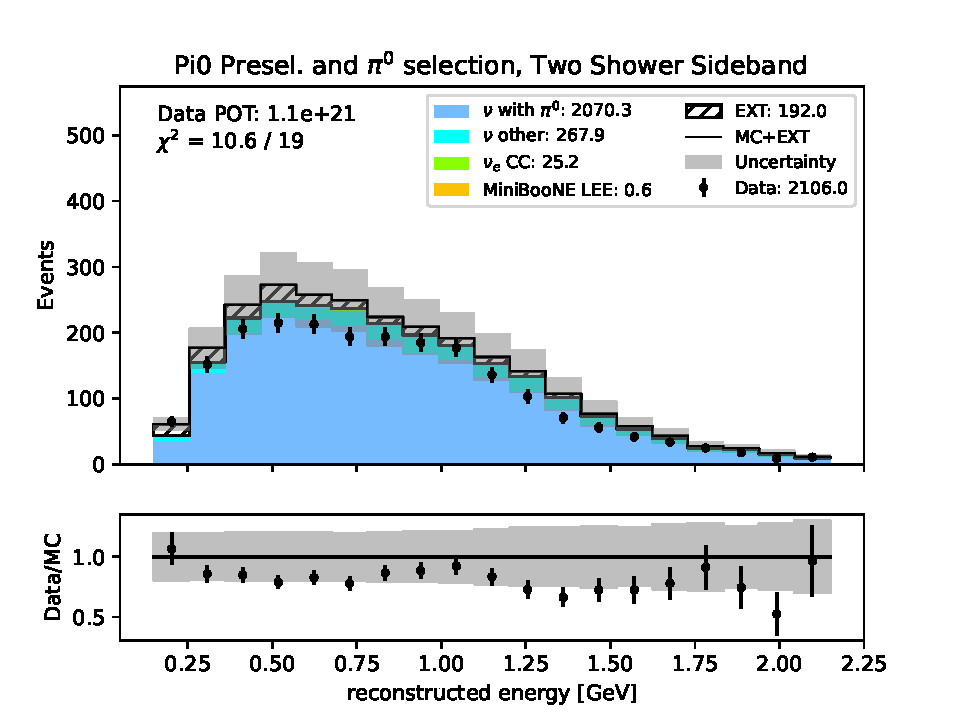
\includegraphics[width=\linewidth]{technote/Sidebands/Figures/TwoShowerSideband/two_shr_sideband_reco_e_run1234b4c4d5_PI0_PI0.pdf}
        \caption{Reconstructed neutrino energy, runs 1-5.}
    \end{subfigure}
    \caption{Data and MC simulation comparisons after applying the full $\pi^0$ selection from Appendix~\ref{appendix:Pi0Selection} to data from the two shower sideband.}
    \label{fig:Pi0Sideband}
\end{figure}

\subsection{Near and Far Sidebands}
\label{sec:NearAndFarSideband}

The far sidebands are obtained by applying the full event selections for the signal channels, described in Appendix~\ref{appendix:1e0pSelection} and~\ref{appendix:1eNpSelection}, with blindness achieved through inversion of the BDT cuts, or only selecting events with reconstructed energies above the signal region. This approach is illustrated in Figure~\ref{fig:SidebandStructure}, in which the palest green squares represent the far sideband, while the slightly darker green is the near sideband. The definitions are slightly different for the 1e0p and 1eNp event selections. The variables that will be examined are the BDT response scores, and the reconstructed neutrino energy.

\begin{figure}[H]
    \centering
    \begin{subfigure}{0.5\linewidth}
        \includegraphics[width=\linewidth]{technote/Sidebands/Figures/ZpNearAndFarSidebands.pdf}
        \caption{For the 1e0p selection.}
    \end{subfigure}%
    \begin{subfigure}{0.5\linewidth}
        \includegraphics[width=\linewidth]{technote/Sidebands/Figures/NpNearAndFarSidebands.pdf}
        \caption{For the 1eNp selection.}
    \end{subfigure}
    \caption{The structures of the near and far sidebands for the two event selections. The palest green regions represent the far sidebands, while the slightly darker green represents the near sidebands.}
    \label{fig:SidebandStructure}
\end{figure}

\subsection{High Energy Sidebands}
\label{sec:HighEnergySidebands}

The first set of sub-sidebands to inspect is obtained by selecting the high energy regions of the two far sidebands. These are defined in the case of the 1eNp selection as events with a reconstructed energy greater than 1.05~GeV and in the case of the 1e0p, events with reconstructed energies above 0.90~GeV. These selections are illustrated in Figure~\ref{fig:HighEnergySideband}.

\begin{figure}[H]
    \centering
    \begin{subfigure}{0.5\linewidth}
        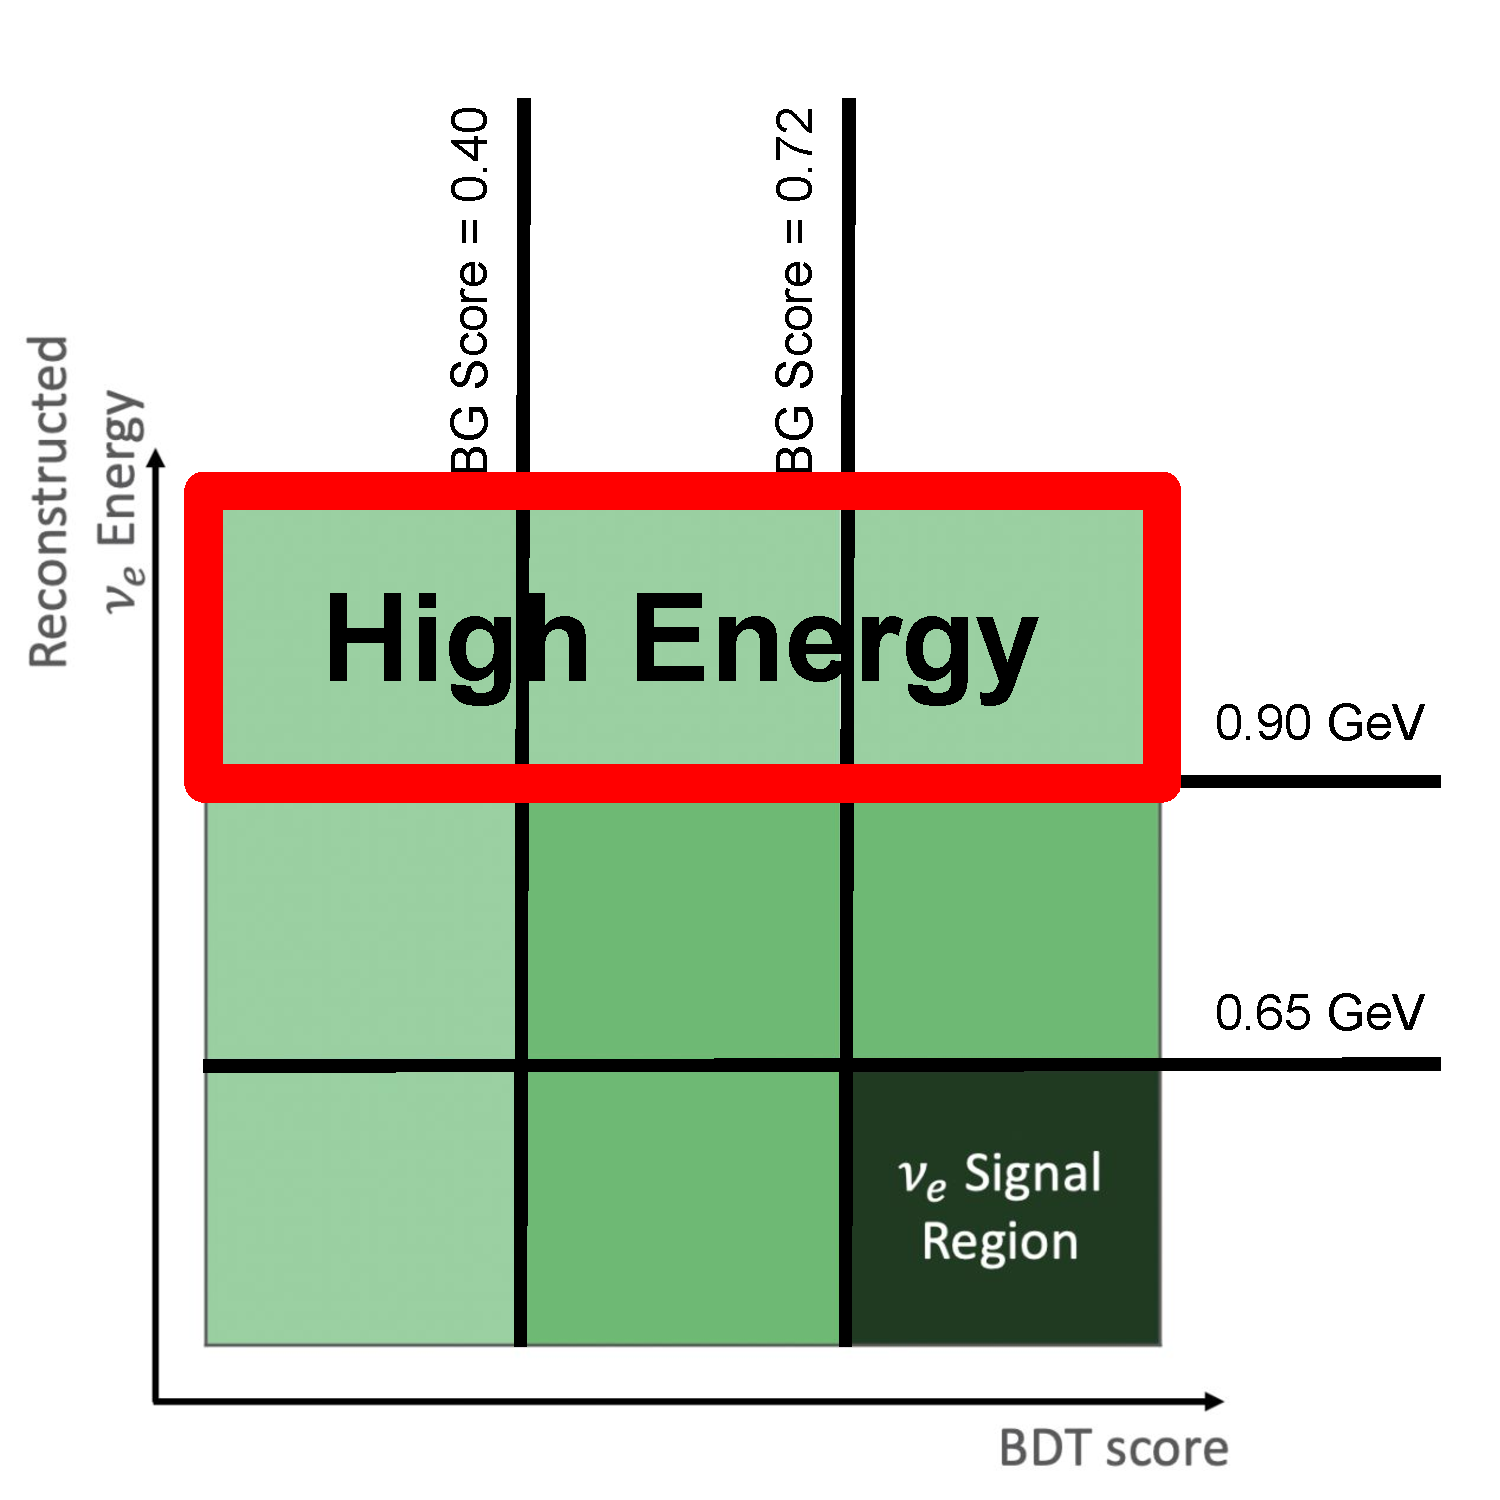
\includegraphics[width=\linewidth]{technote/Sidebands/Figures/FarSideband/ZpHighEnergySideband.pdf}
        \caption{For the 1e0p selection.}
    \end{subfigure}%
    \begin{subfigure}{0.5\linewidth}
        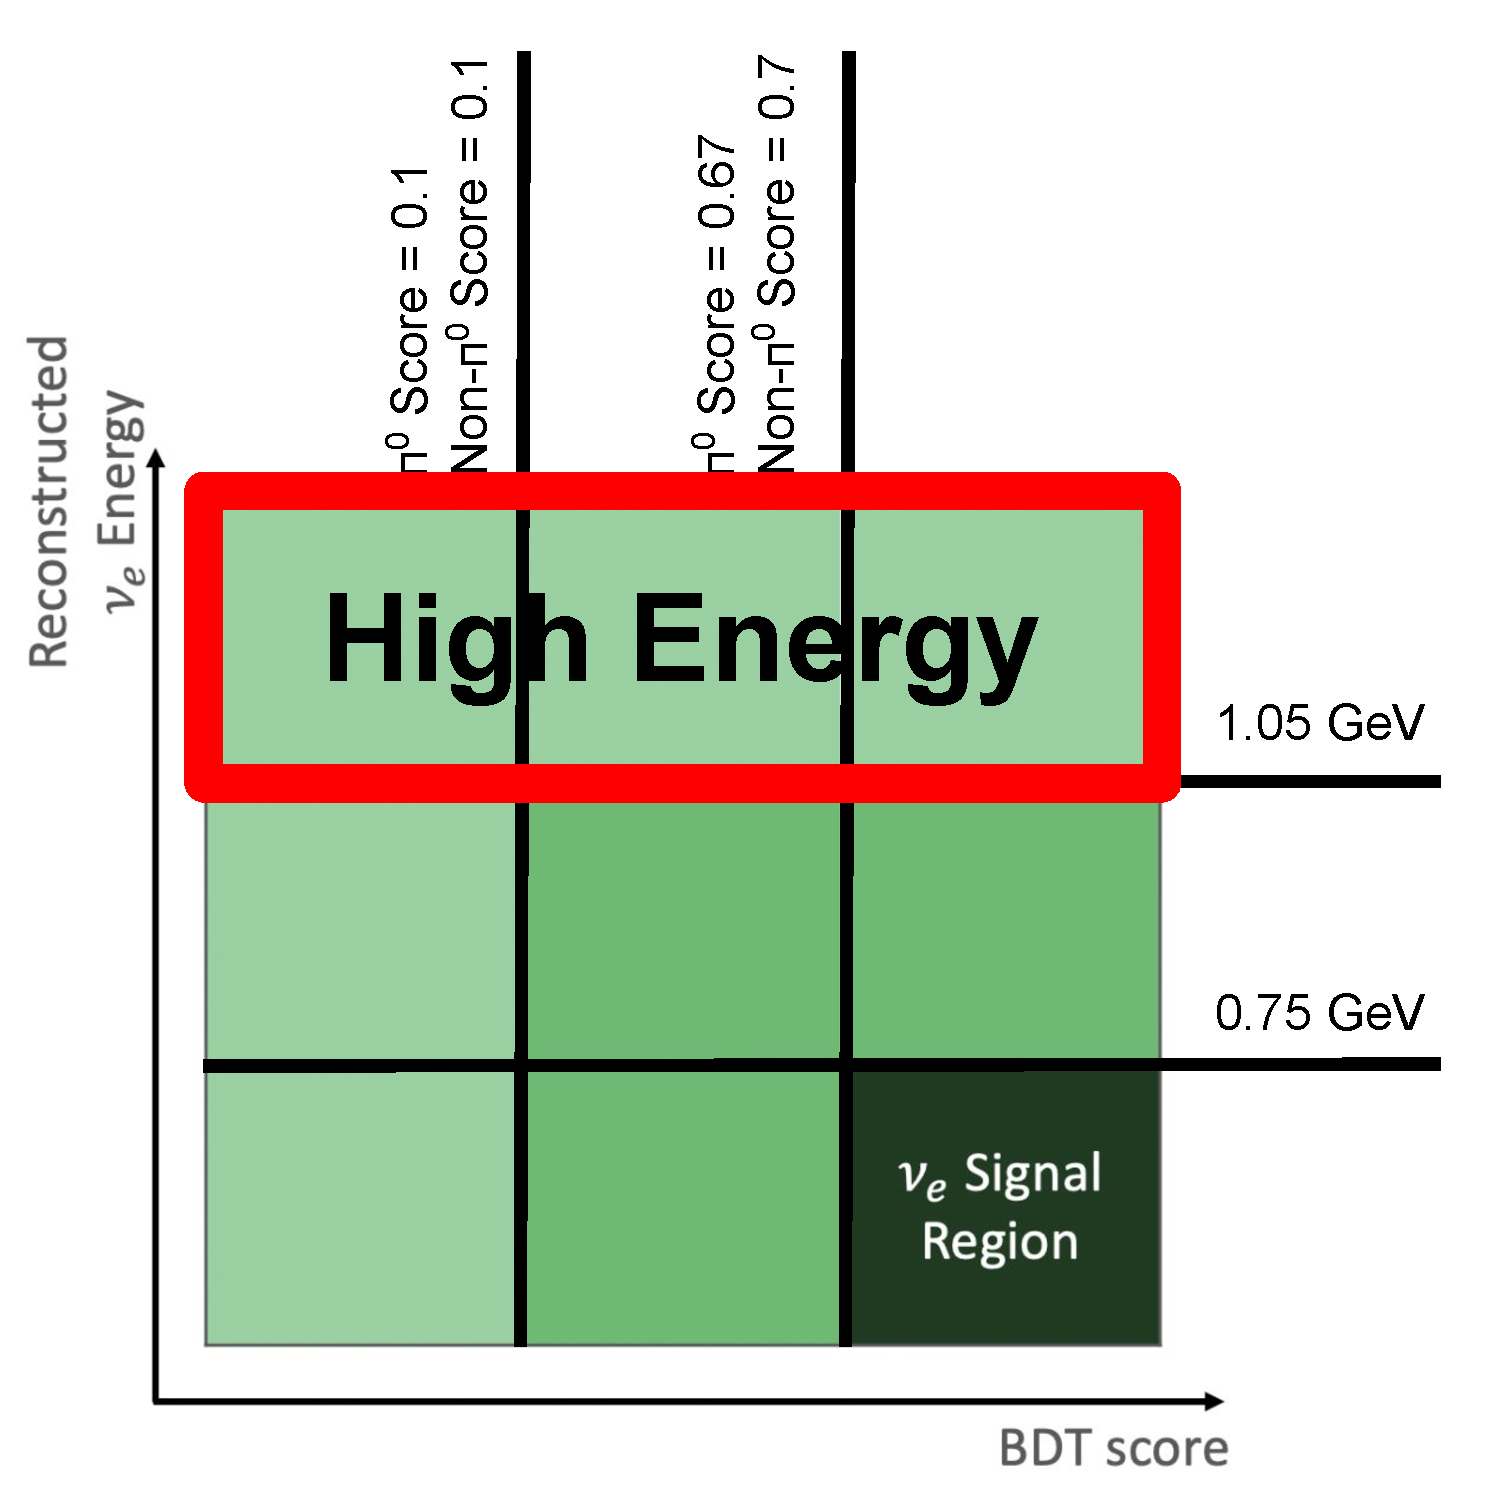
\includegraphics[width=\linewidth]{technote/Sidebands/Figures/FarSideband/NpHighEnergySideband.pdf}
        \caption{For the 1eNp selection.}
    \end{subfigure}
    \caption{The high energy sidebands.}
    \label{fig:HighEnergySideband}
\end{figure}

\begin{figure}[H]
    \centering
    \begin{subfigure}{0.33\linewidth}
    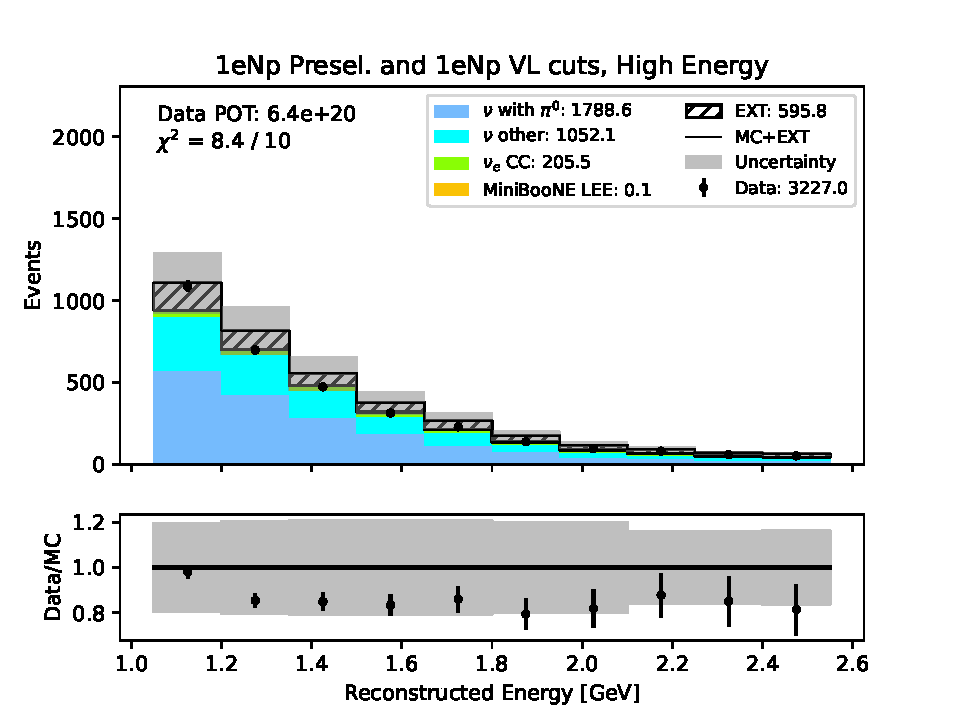
\includegraphics[width=\linewidth]{technote/Sidebands/Figures/FarSideband/far_sideband_reco_e_run123_NP_NP_HIGH_ENERGY.pdf}
    \caption{$\nu_e$ preselection, runs 1-3.}
    \end{subfigure}%
    \begin{subfigure}{0.33\linewidth}
    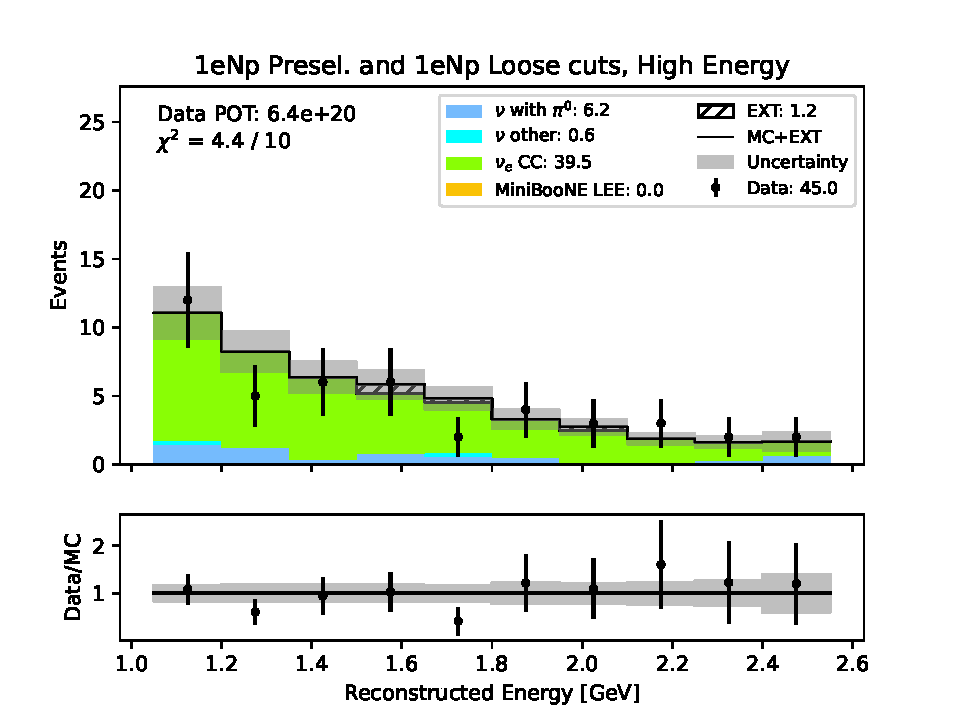
\includegraphics[width=\linewidth]{technote/Sidebands/Figures/FarSideband/far_sideband_reco_e_run123_NP_NPL_HIGH_ENERGY.pdf}
    \caption{1eNp loose selection, runs 1-3.}
    \end{subfigure}%
    \begin{subfigure}{0.33\linewidth}
    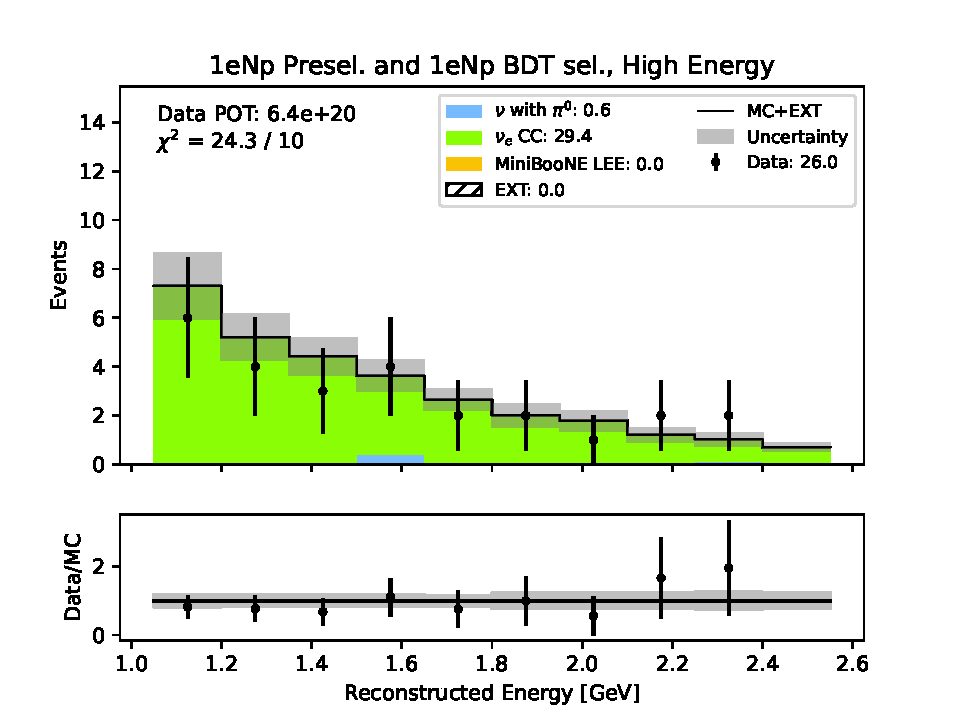
\includegraphics[width=\linewidth]{technote/Sidebands/Figures/FarSideband/far_sideband_reco_e_run123_NP_NPBDT_HIGH_ENERGY.pdf}
    \caption{1eNp BDT selection, runs 1-3.}
    \end{subfigure}
    \begin{subfigure}{0.33\linewidth}
    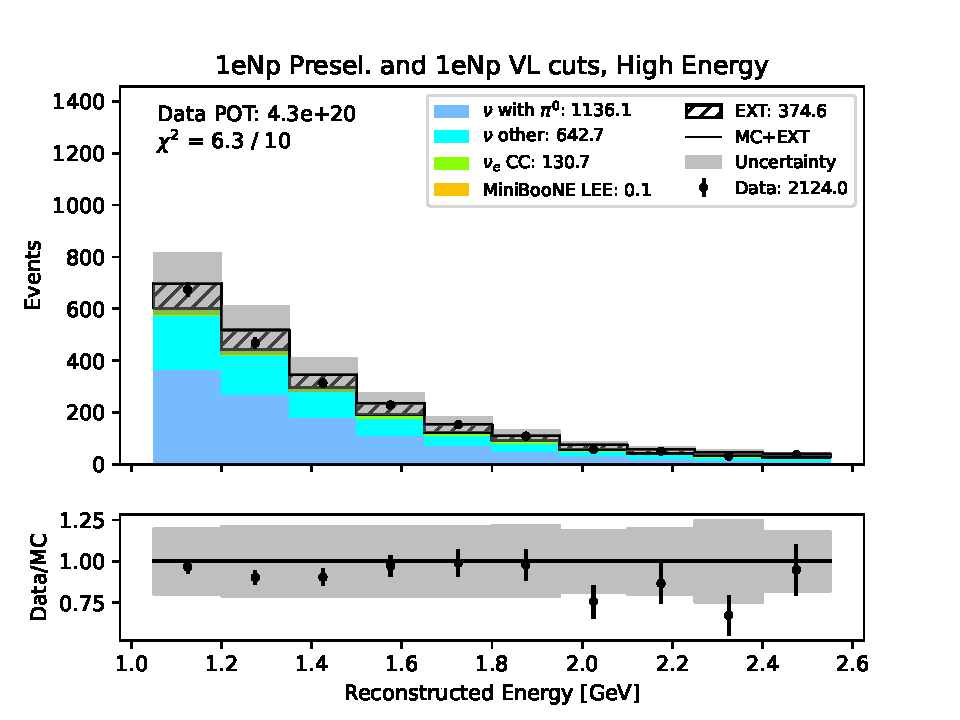
\includegraphics[width=\linewidth]{technote/Sidebands/Figures/FarSideband/far_sideband_reco_e_run4b4c4d5_NP_NP_HIGH_ENERGY.pdf}
    \caption{$\nu_e$ preselection, runs 4-5.}
    \end{subfigure}%
    \begin{subfigure}{0.33\linewidth}
    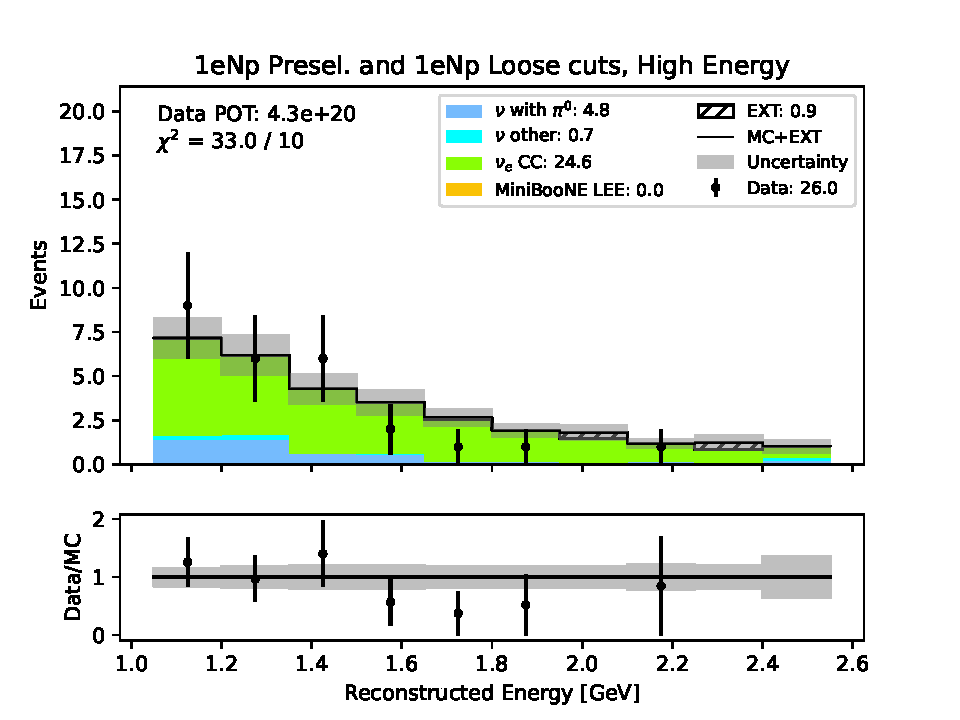
\includegraphics[width=\linewidth]{technote/Sidebands/Figures/FarSideband/far_sideband_reco_e_run4b4c4d5_NP_NPL_HIGH_ENERGY.pdf}
    \caption{1eNp loose selection, runs 4-5.}
    \end{subfigure}%
    \begin{subfigure}{0.33\linewidth}
    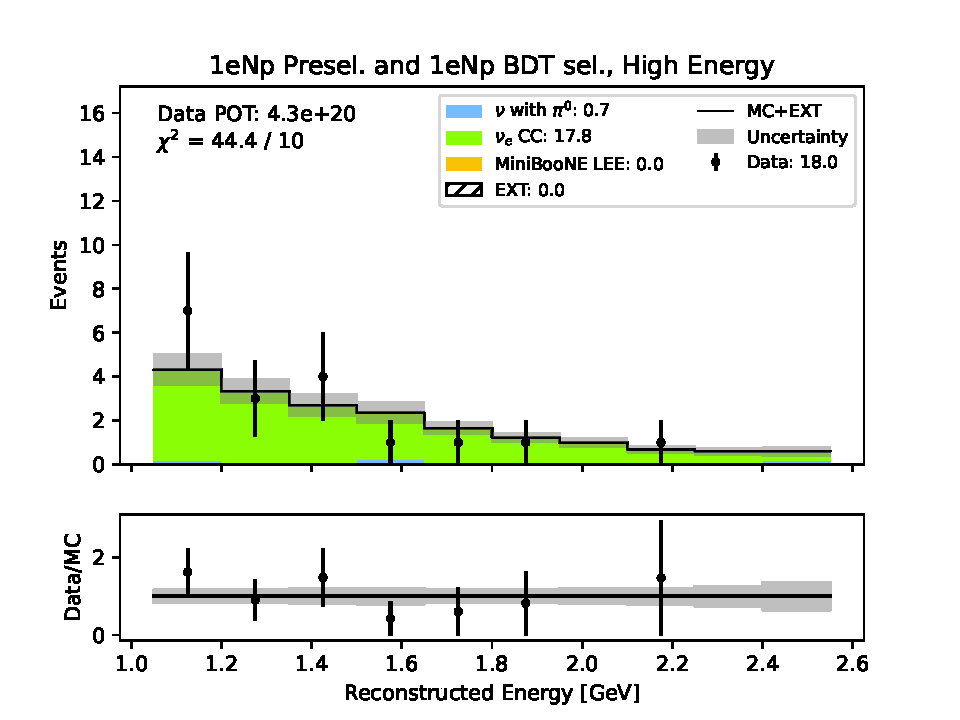
\includegraphics[width=\linewidth]{technote/Sidebands/Figures/FarSideband/far_sideband_reco_e_run4b4c4d5_NP_NPBDT_HIGH_ENERGY.pdf}
    \caption{1eNp BDT selection, runs 4-5.}
    \end{subfigure}
    \begin{subfigure}{0.33\linewidth}
    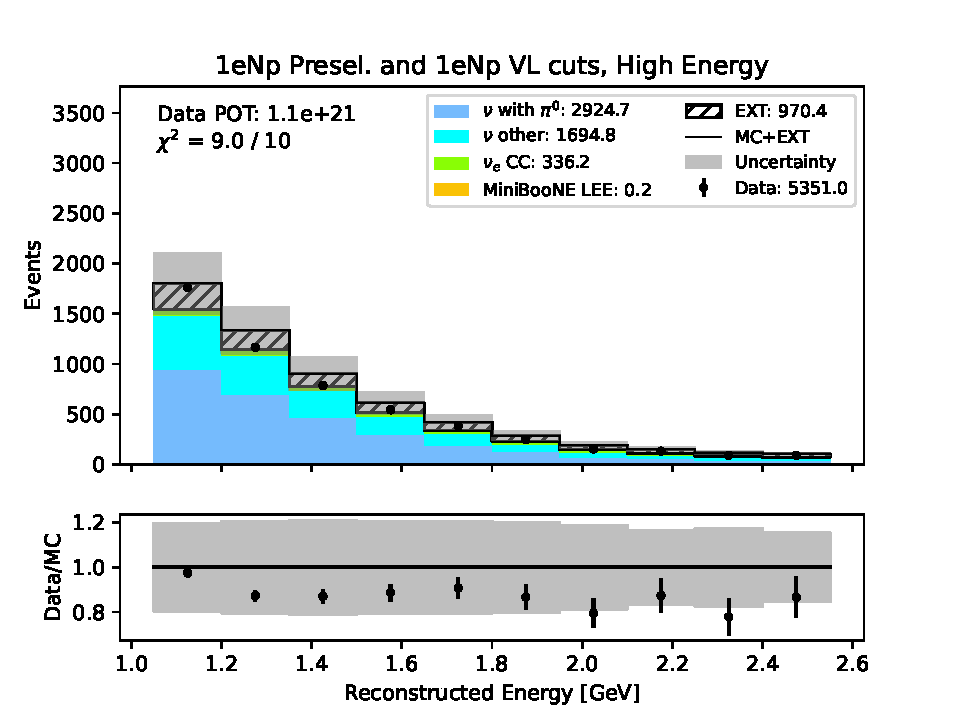
\includegraphics[width=\linewidth]{technote/Sidebands/Figures/FarSideband/far_sideband_reco_e_run1234b4c4d5_NP_NP_HIGH_ENERGY.pdf}
    \caption{$\nu_e$ preselection, runs 1-5.}
    \end{subfigure}%
    \begin{subfigure}{0.33\linewidth}
    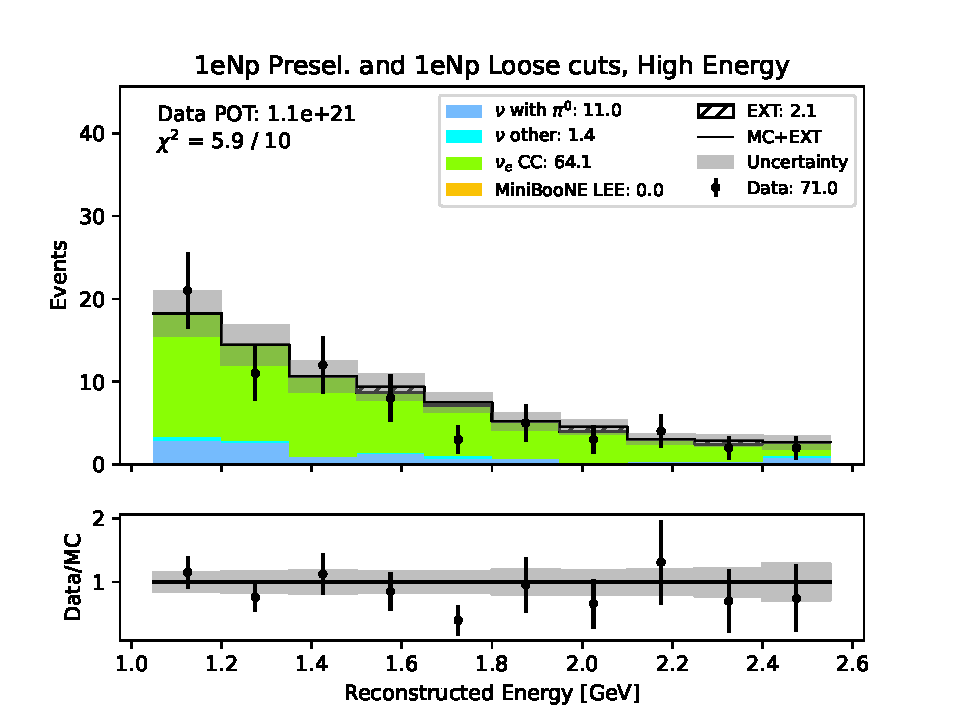
\includegraphics[width=\linewidth]{technote/Sidebands/Figures/FarSideband/far_sideband_reco_e_run1234b4c4d5_NP_NPL_HIGH_ENERGY.pdf}
    \caption{1eNp loose selection, runs 1-5.}
    \end{subfigure}%
    \begin{subfigure}{0.33\linewidth}
    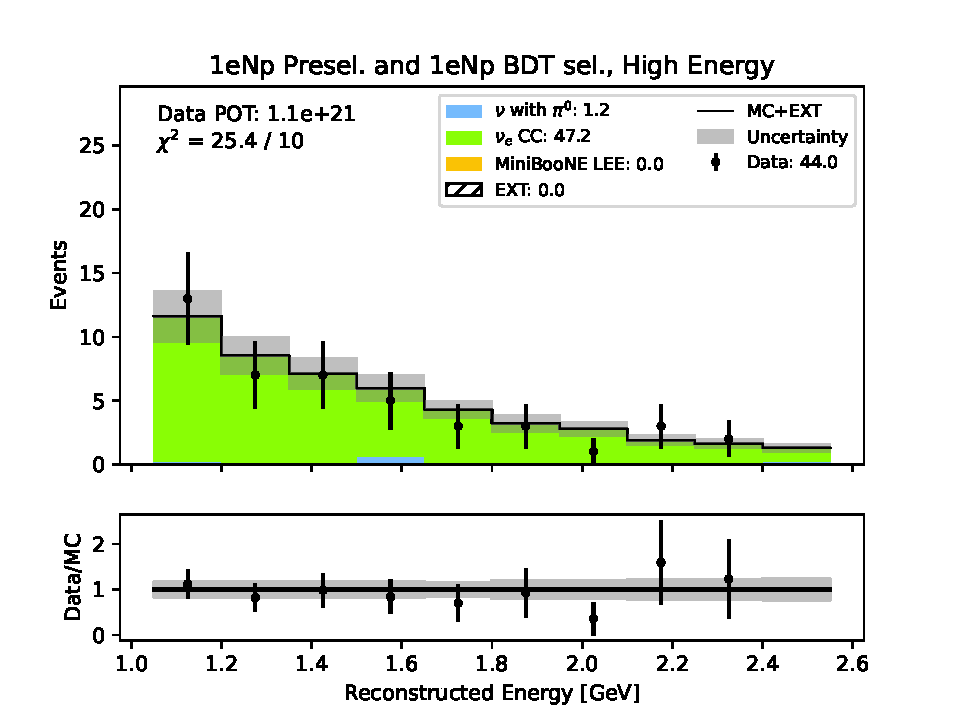
\includegraphics[width=\linewidth]{technote/Sidebands/Figures/FarSideband/far_sideband_reco_e_run1234b4c4d5_NP_NPBDT_HIGH_ENERGY.pdf}
    \caption{1eNp BDT selection, runs 1-5.}
    \end{subfigure}
    \caption{Reconstructed neutrino energy in the 1eNp high energy sideband.}
     \label{fig:HighEnergy1eNp_reco_e}
\end{figure}

\begin{figure}[H]
    \centering
    \begin{subfigure}{0.33\linewidth}
    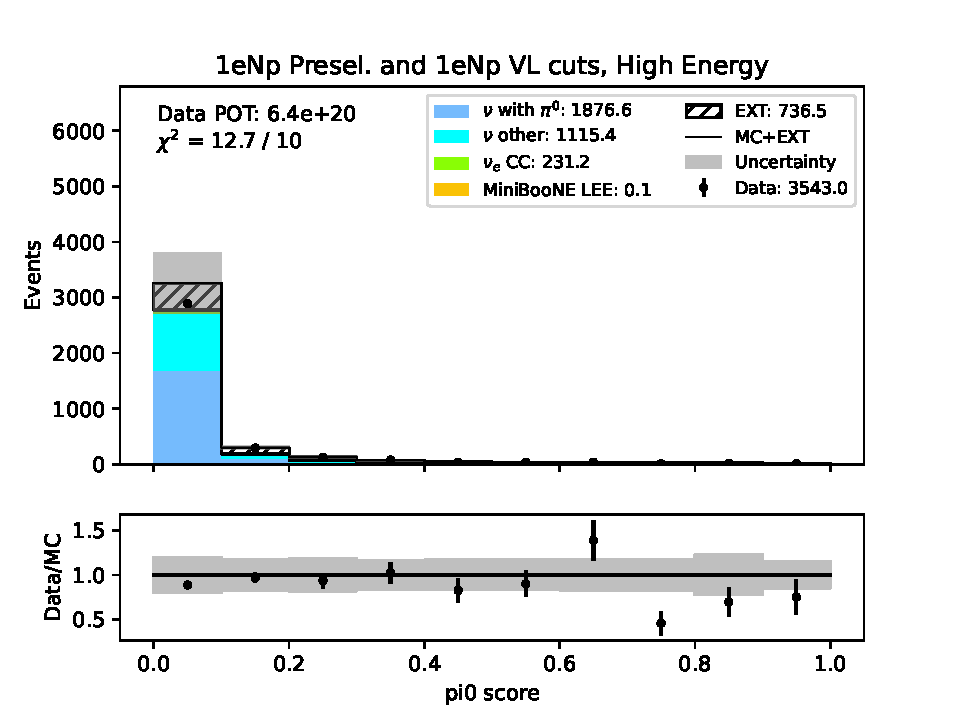
\includegraphics[width=\linewidth]{technote/Sidebands/Figures/FarSideband/far_sideband_pi0_score_run123_NP_NP_HIGH_ENERGY.pdf}
    \caption{$\nu_e$ preselection, runs 1-3.}
    \end{subfigure}%
    \begin{subfigure}{0.33\linewidth}
    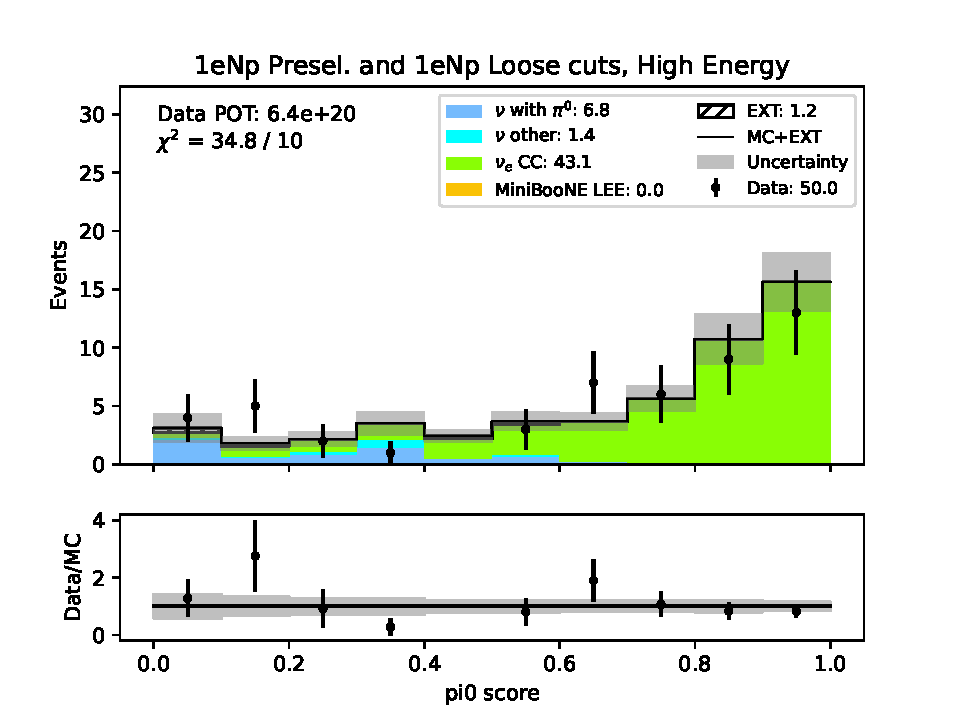
\includegraphics[width=\linewidth]{technote/Sidebands/Figures/FarSideband/far_sideband_pi0_score_run123_NP_NPL_HIGH_ENERGY.pdf}
    \caption{1eNp loose selection, runs 1-3.}
    \end{subfigure}%
    \begin{subfigure}{0.33\linewidth}
    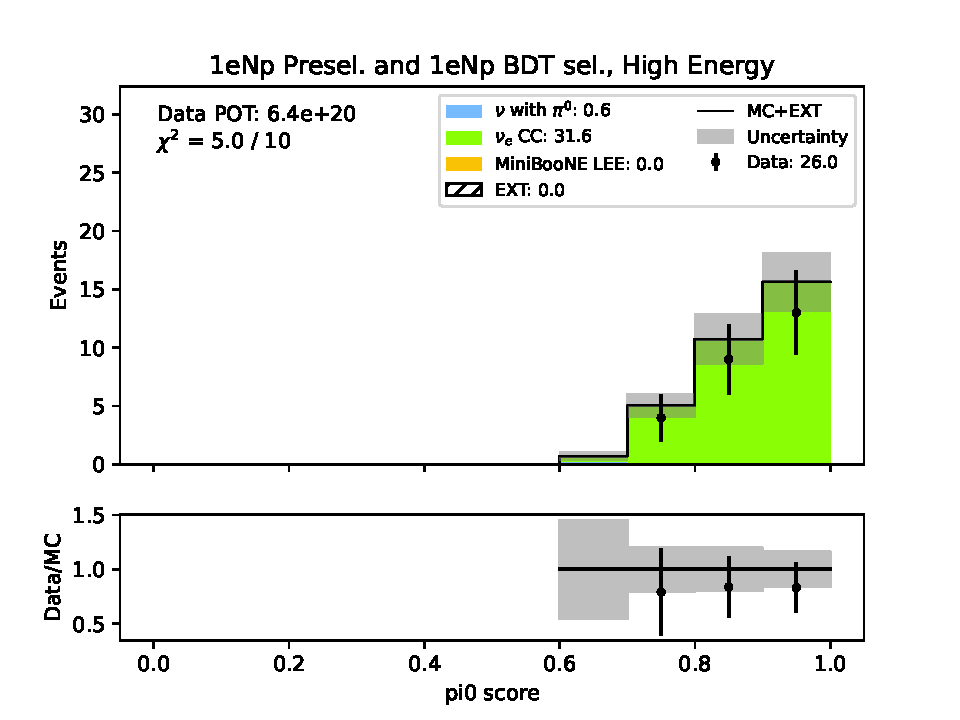
\includegraphics[width=\linewidth]{technote/Sidebands/Figures/FarSideband/far_sideband_pi0_score_run123_NP_NPBDT_HIGH_ENERGY.pdf}
    \caption{1eNp BDT selection, runs 1-3.}
    \end{subfigure}
    \begin{subfigure}{0.33\linewidth}
    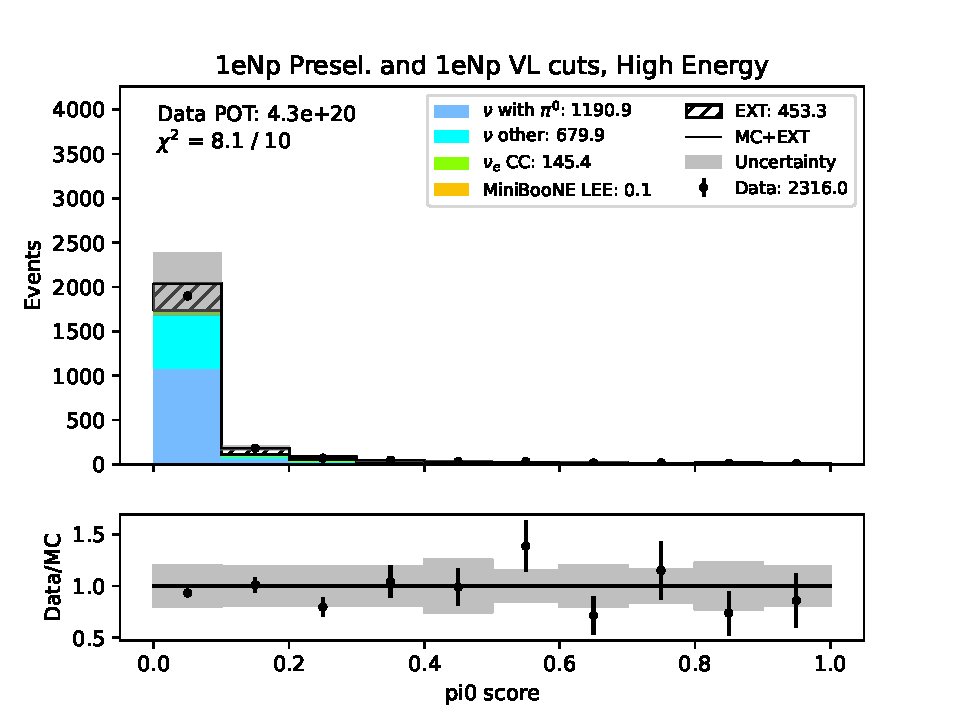
\includegraphics[width=\linewidth]{technote/Sidebands/Figures/FarSideband/far_sideband_pi0_score_run4b4c4d5_NP_NP_HIGH_ENERGY.pdf}
    \caption{$\nu_e$ preselection, runs 4-5.}
    \end{subfigure}%
    \begin{subfigure}{0.33\linewidth}
    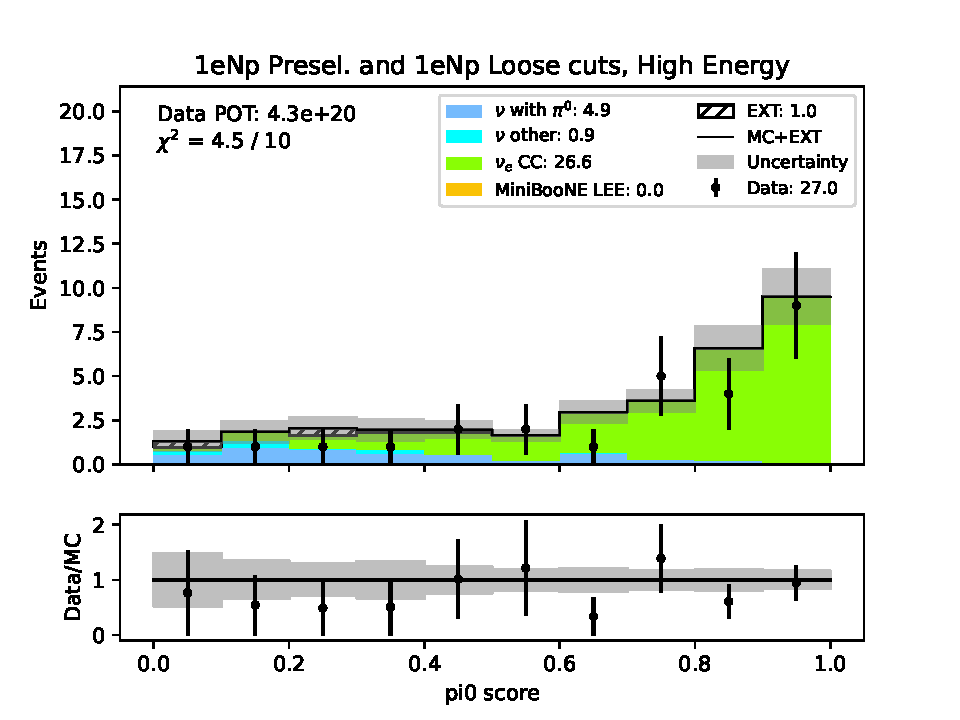
\includegraphics[width=\linewidth]{technote/Sidebands/Figures/FarSideband/far_sideband_pi0_score_run4b4c4d5_NP_NPL_HIGH_ENERGY.pdf}
    \caption{1eNp loose selection, runs 4-5.}
    \end{subfigure}%
    \begin{subfigure}{0.33\linewidth}
    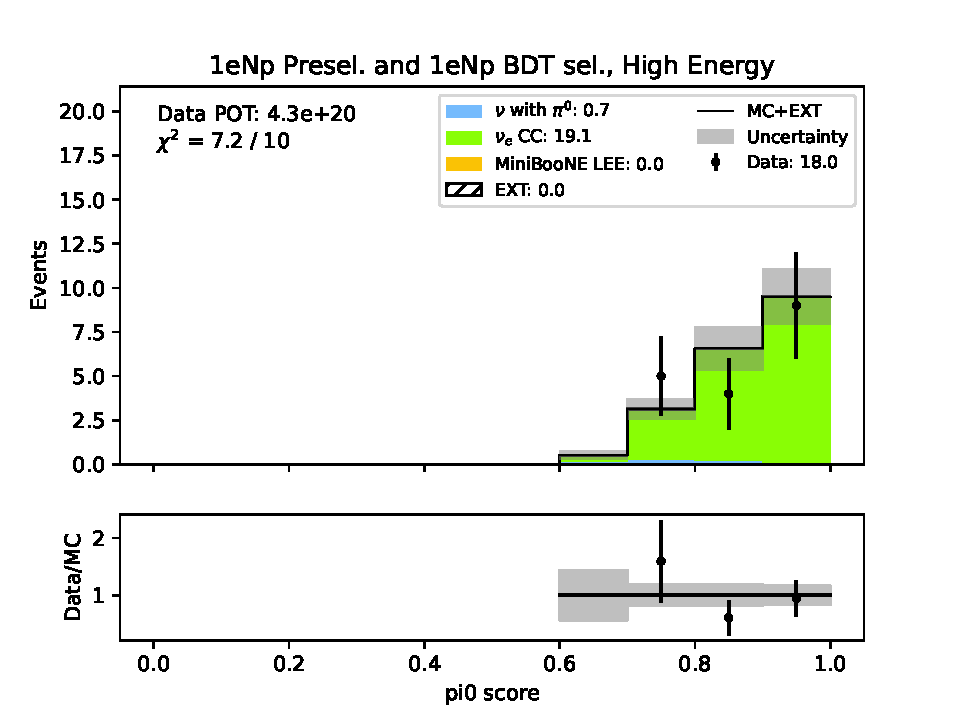
\includegraphics[width=\linewidth]{technote/Sidebands/Figures/FarSideband/far_sideband_pi0_score_run4b4c4d5_NP_NPBDT_HIGH_ENERGY.pdf}
    \caption{1eNp BDT selection, runs 4-5.}
    \end{subfigure}
    \begin{subfigure}{0.33\linewidth}
    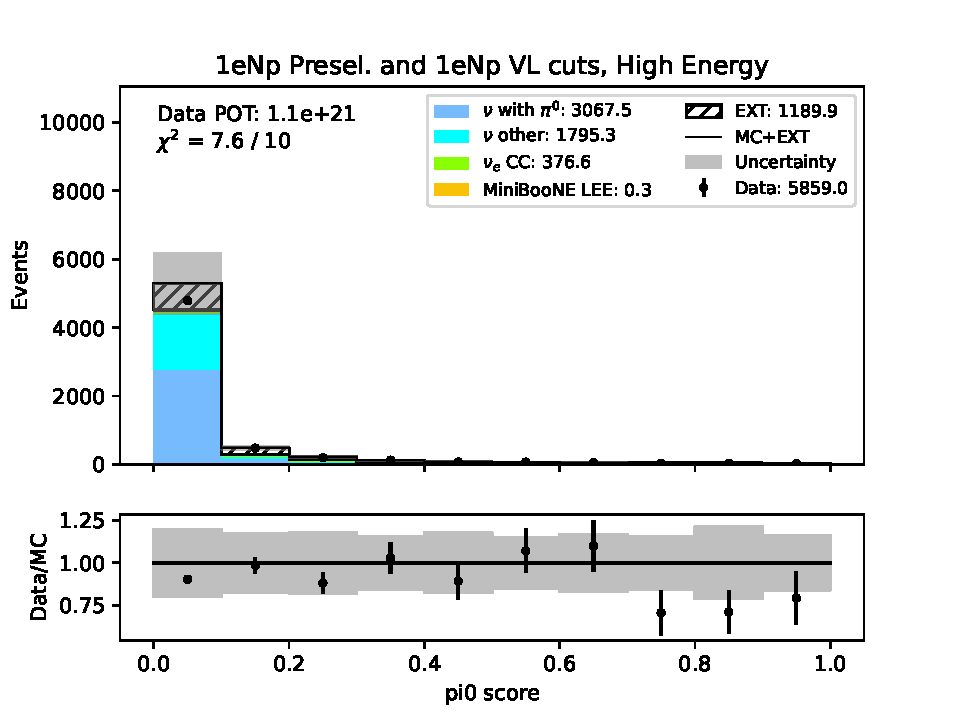
\includegraphics[width=\linewidth]{technote/Sidebands/Figures/FarSideband/far_sideband_pi0_score_run1234b4c4d5_NP_NP_HIGH_ENERGY.pdf}
    \caption{$\nu_e$ preselection, runs 1-5.}
    \end{subfigure}%
    \begin{subfigure}{0.33\linewidth}
    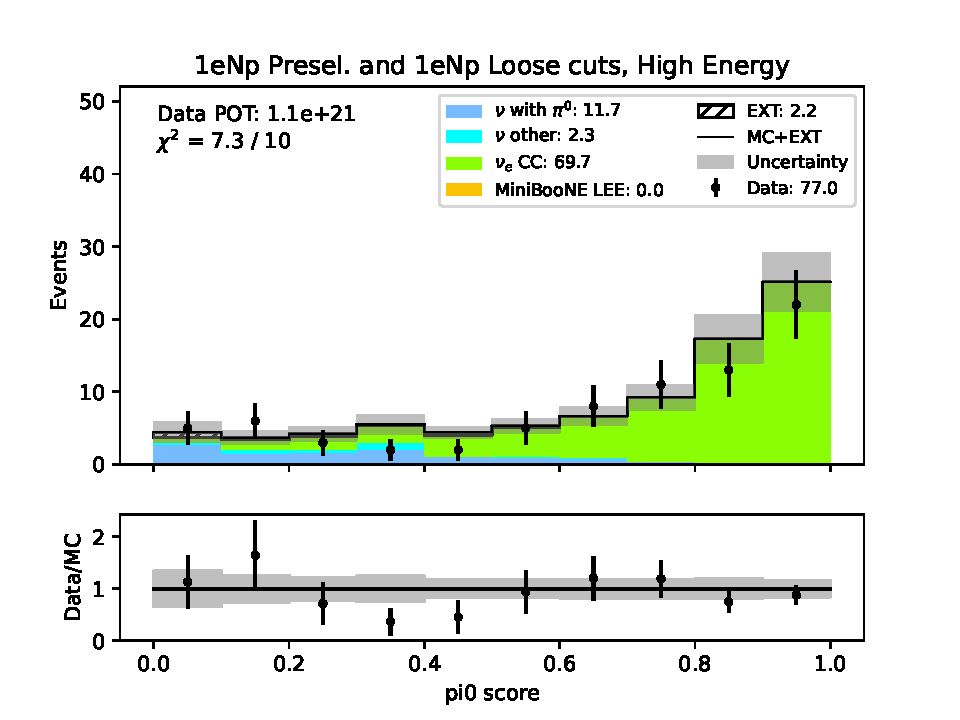
\includegraphics[width=\linewidth]{technote/Sidebands/Figures/FarSideband/far_sideband_pi0_score_run1234b4c4d5_NP_NPL_HIGH_ENERGY.pdf}
    \caption{1eNp loose selection, runs 1-5.}
    \end{subfigure}%
    \begin{subfigure}{0.33\linewidth}
    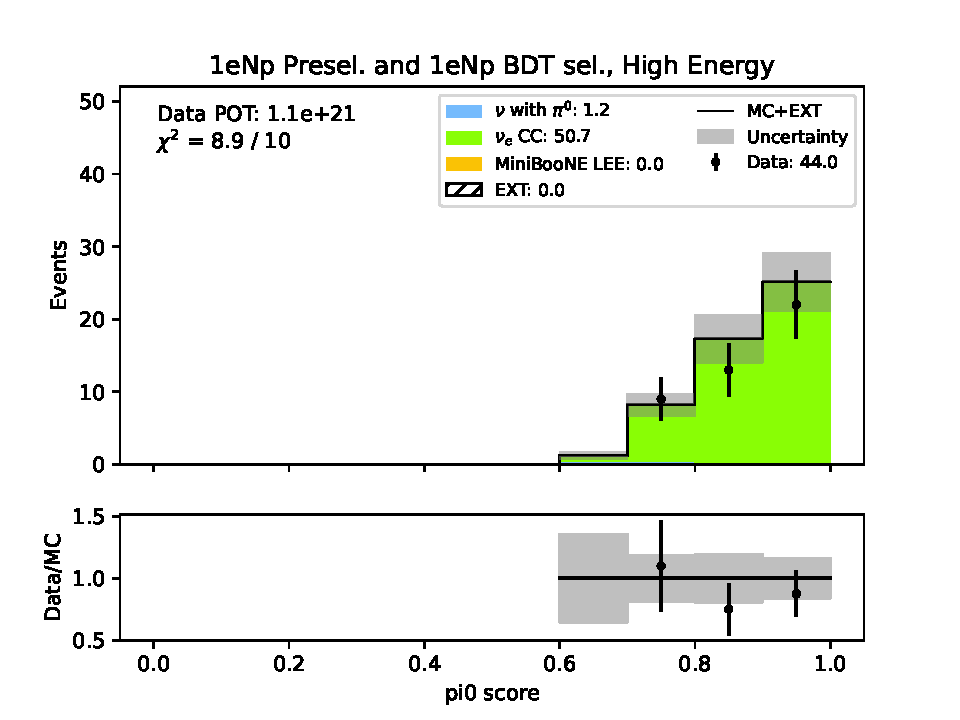
\includegraphics[width=\linewidth]{technote/Sidebands/Figures/FarSideband/far_sideband_pi0_score_run1234b4c4d5_NP_NPBDT_HIGH_ENERGY.pdf}
    \caption{1eNp BDT selection, runs 1-5.}
    \end{subfigure}
    \caption{Reconstructed neutrino energy in the 1eNp high energy sideband.}
    \label{fig:HighEnergy1eNp_pi0_score}
\end{figure}

\begin{figure}[H]
    \centering
    \begin{subfigure}{0.33\linewidth}
    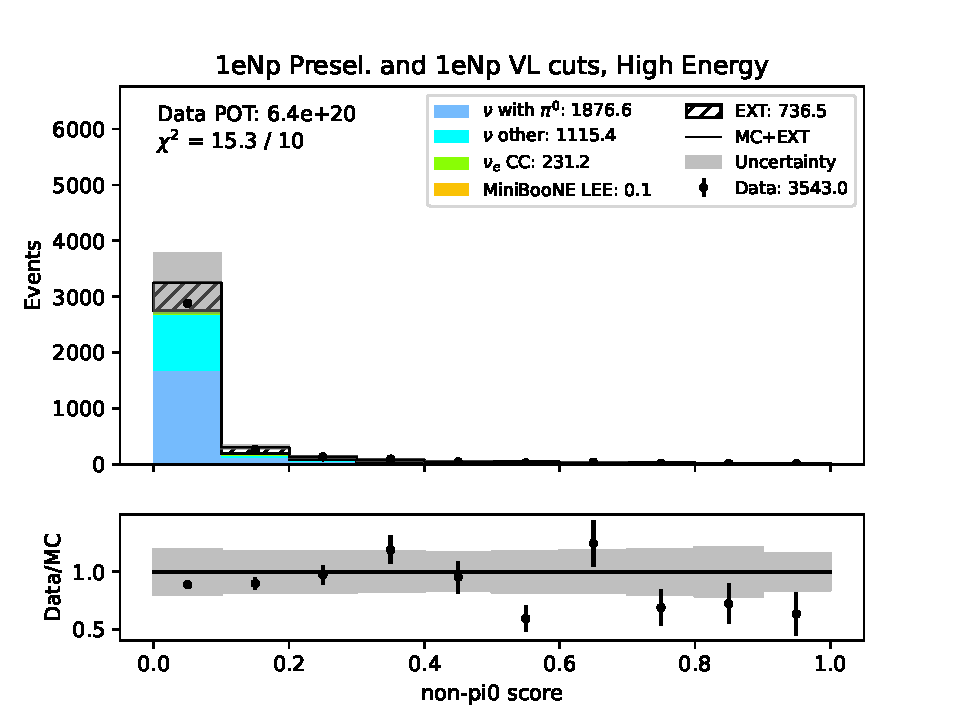
\includegraphics[width=\linewidth]{technote/Sidebands/Figures/FarSideband/far_sideband_nonpi0_score_run123_NP_NP_HIGH_ENERGY.pdf}
    \caption{$\nu_e$ preselection, runs 1-3.}
    \end{subfigure}%
    \begin{subfigure}{0.33\linewidth}
    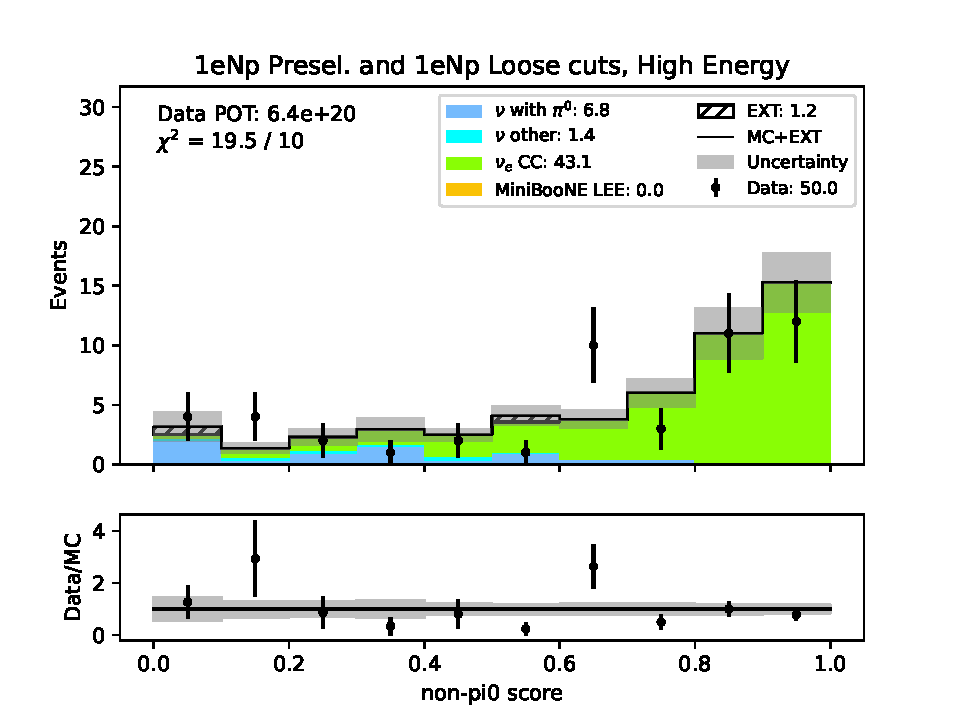
\includegraphics[width=\linewidth]{technote/Sidebands/Figures/FarSideband/far_sideband_nonpi0_score_run123_NP_NPL_HIGH_ENERGY.pdf}
    \caption{1eNp loose selection, runs 1-3.}
    \end{subfigure}%
    \begin{subfigure}{0.33\linewidth}
    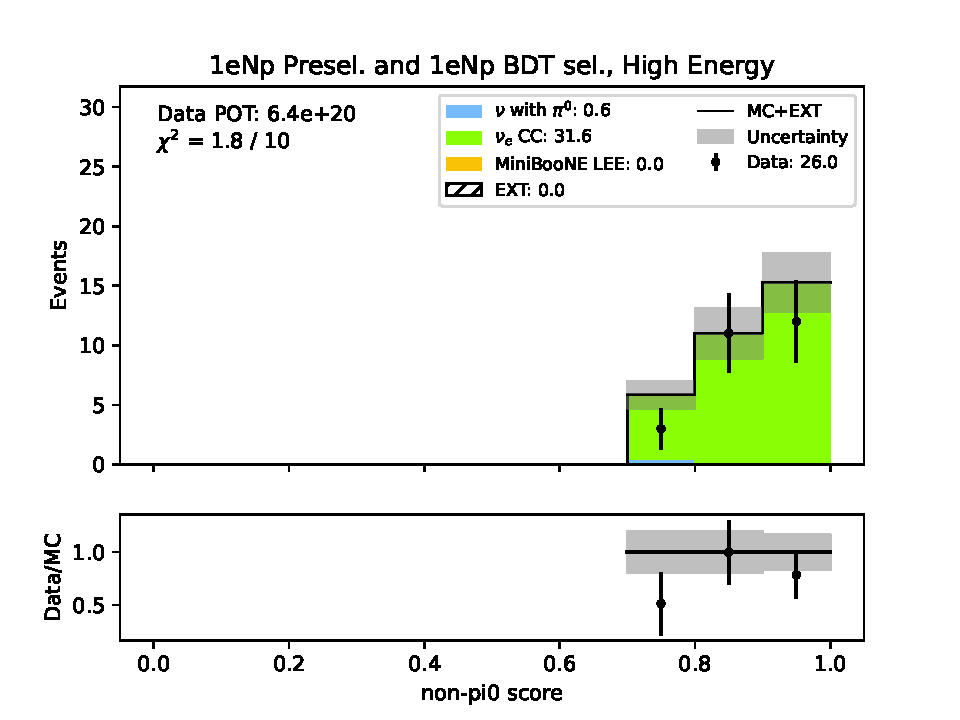
\includegraphics[width=\linewidth]{technote/Sidebands/Figures/FarSideband/far_sideband_nonpi0_score_run123_NP_NPBDT_HIGH_ENERGY.pdf}
    \caption{1eNp BDT selection, runs 1-3.}
    \end{subfigure}
    \begin{subfigure}{0.33\linewidth}
    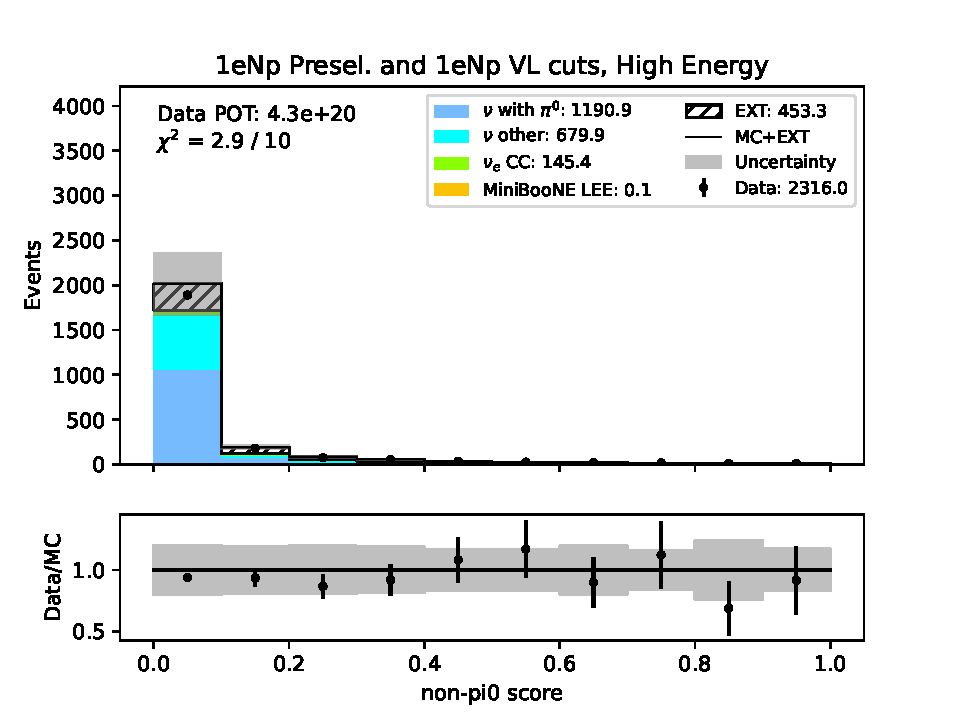
\includegraphics[width=\linewidth]{technote/Sidebands/Figures/FarSideband/far_sideband_nonpi0_score_run4b4c4d5_NP_NP_HIGH_ENERGY.pdf}
    \caption{$\nu_e$ preselection, runs 4-5.}
    \end{subfigure}%
    \begin{subfigure}{0.33\linewidth}
    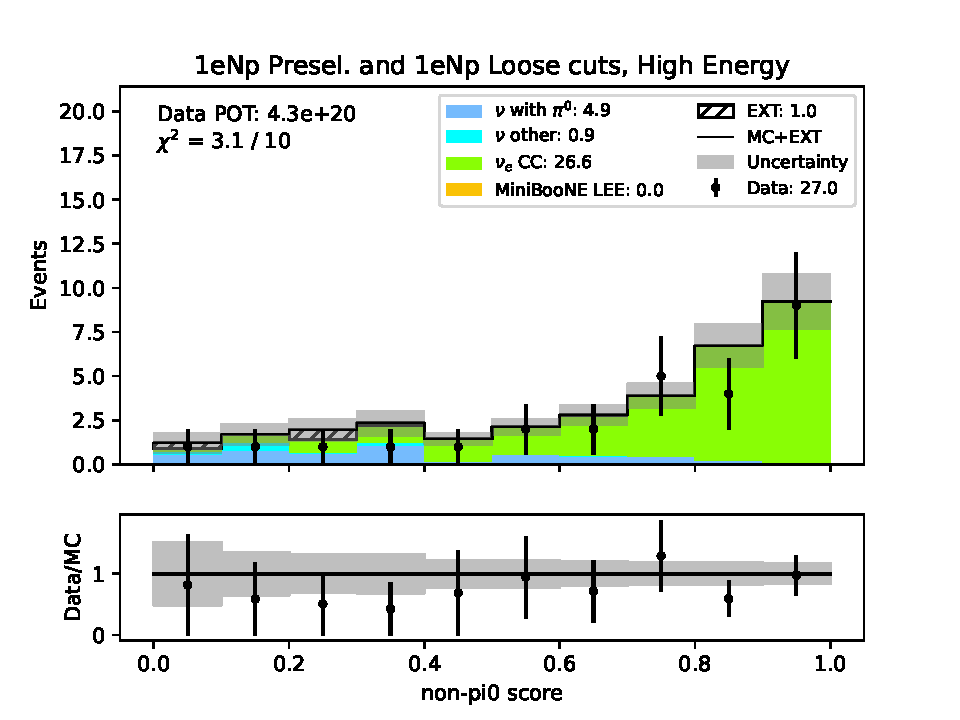
\includegraphics[width=\linewidth]{technote/Sidebands/Figures/FarSideband/far_sideband_nonpi0_score_run4b4c4d5_NP_NPL_HIGH_ENERGY.pdf}
    \caption{1eNp loose selection, runs 4-5.}
    \end{subfigure}%
    \begin{subfigure}{0.33\linewidth}
    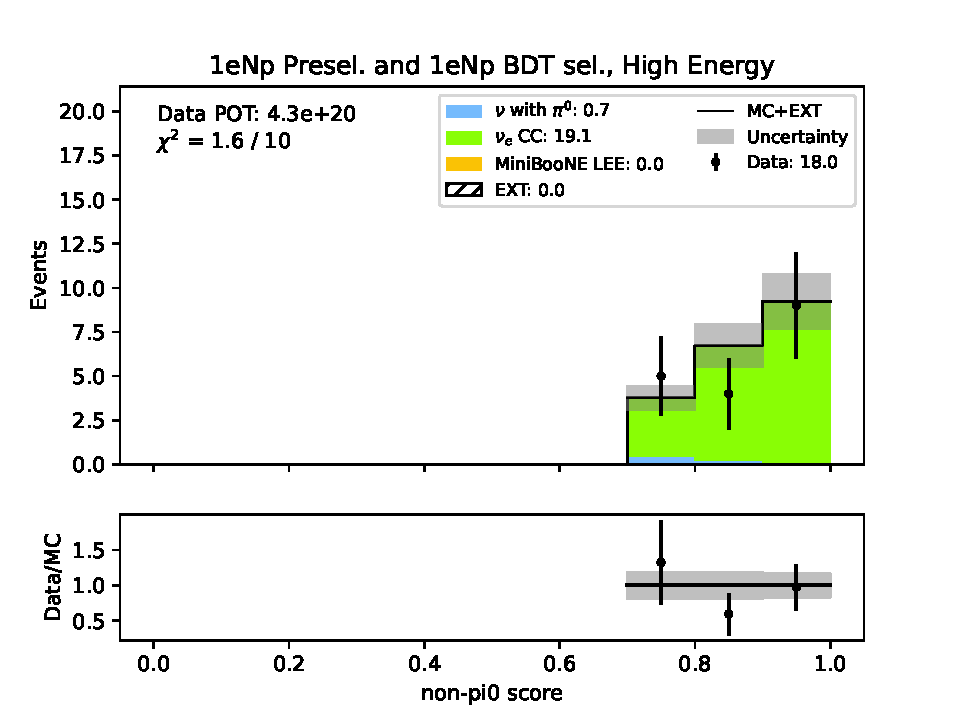
\includegraphics[width=\linewidth]{technote/Sidebands/Figures/FarSideband/far_sideband_nonpi0_score_run4b4c4d5_NP_NPBDT_HIGH_ENERGY.pdf}
    \caption{1eNp BDT selection, runs 4-5.}
    \end{subfigure}
    \begin{subfigure}{0.33\linewidth}
    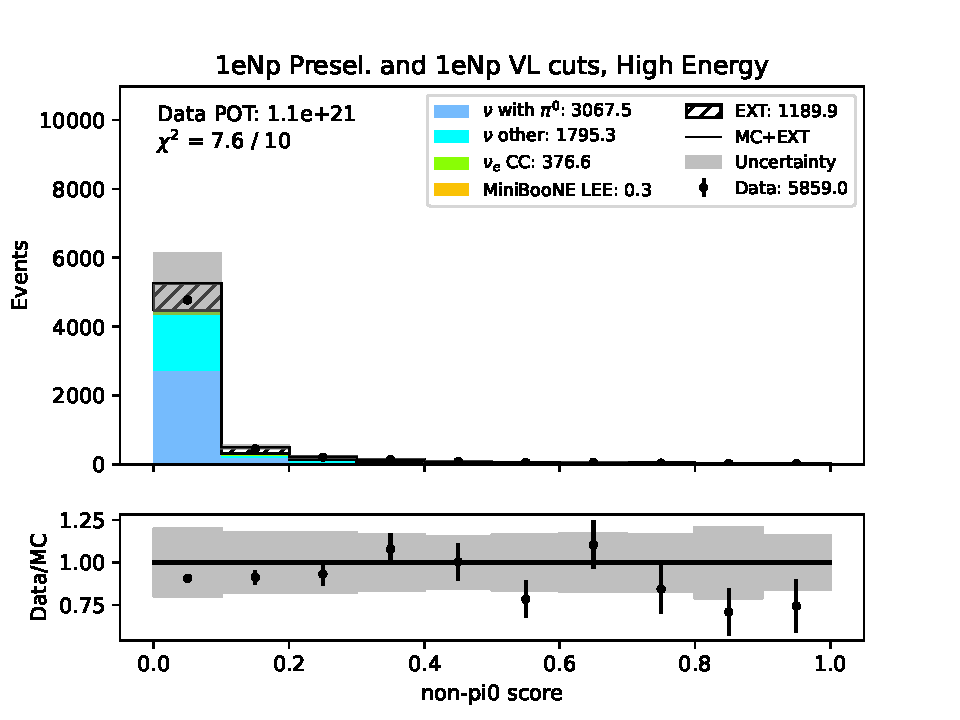
\includegraphics[width=\linewidth]{technote/Sidebands/Figures/FarSideband/far_sideband_nonpi0_score_run1234b4c4d5_NP_NP_HIGH_ENERGY.pdf}
    \caption{$\nu_e$ preselection, runs 1-5.}
    \end{subfigure}%
    \begin{subfigure}{0.33\linewidth}
    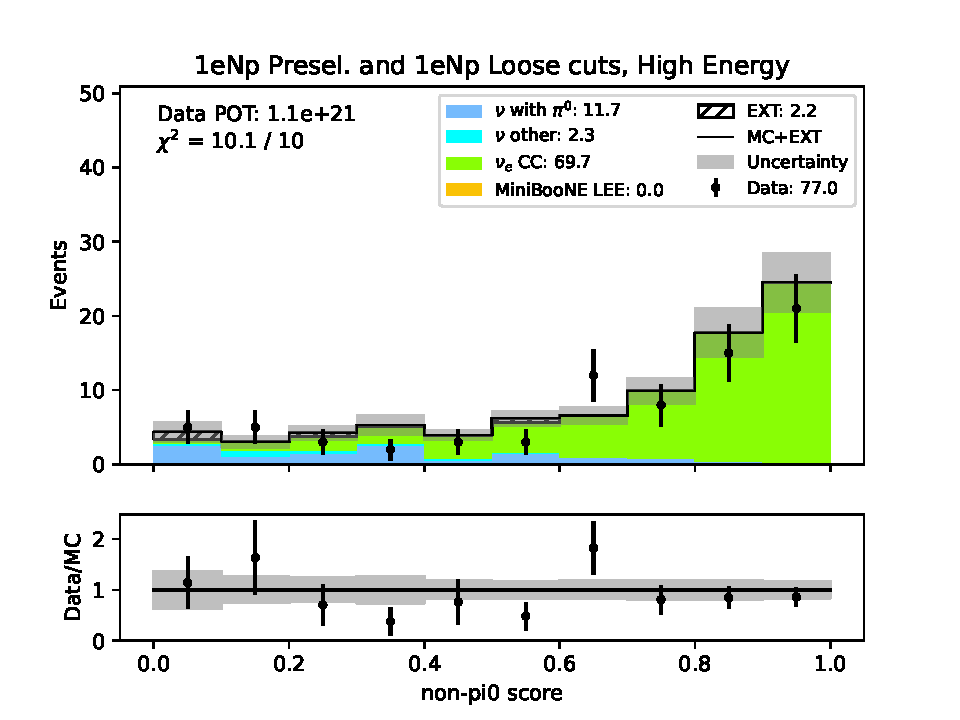
\includegraphics[width=\linewidth]{technote/Sidebands/Figures/FarSideband/far_sideband_nonpi0_score_run1234b4c4d5_NP_NPL_HIGH_ENERGY.pdf}
    \caption{1eNp loose selection, runs 1-5.}
    \end{subfigure}%
    \begin{subfigure}{0.33\linewidth}
    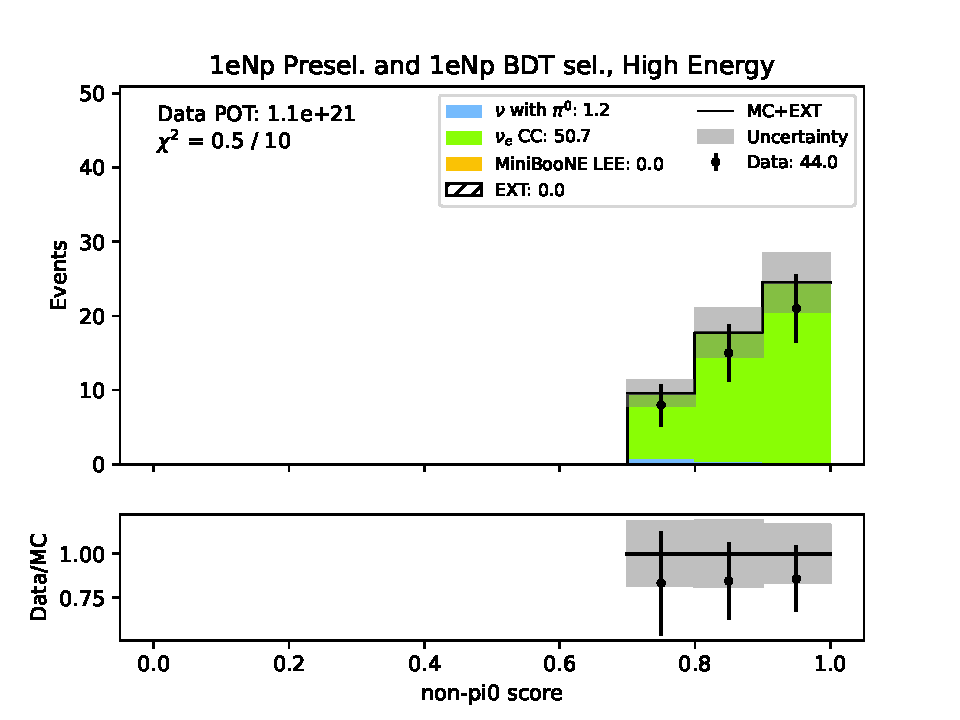
\includegraphics[width=\linewidth]{technote/Sidebands/Figures/FarSideband/far_sideband_nonpi0_score_run1234b4c4d5_NP_NPBDT_HIGH_ENERGY.pdf}
    \caption{1eNp BDT selection, runs 1-5.}
    \end{subfigure}
    \caption{Reconstructed neutrino energy in the 1eNp high energy sideband.}
    \label{fig:HighEnergy1eNp_nonpi0_score}
\end{figure}

\begin{figure}[H]
    \centering
    \begin{subfigure}{0.5\linewidth}
    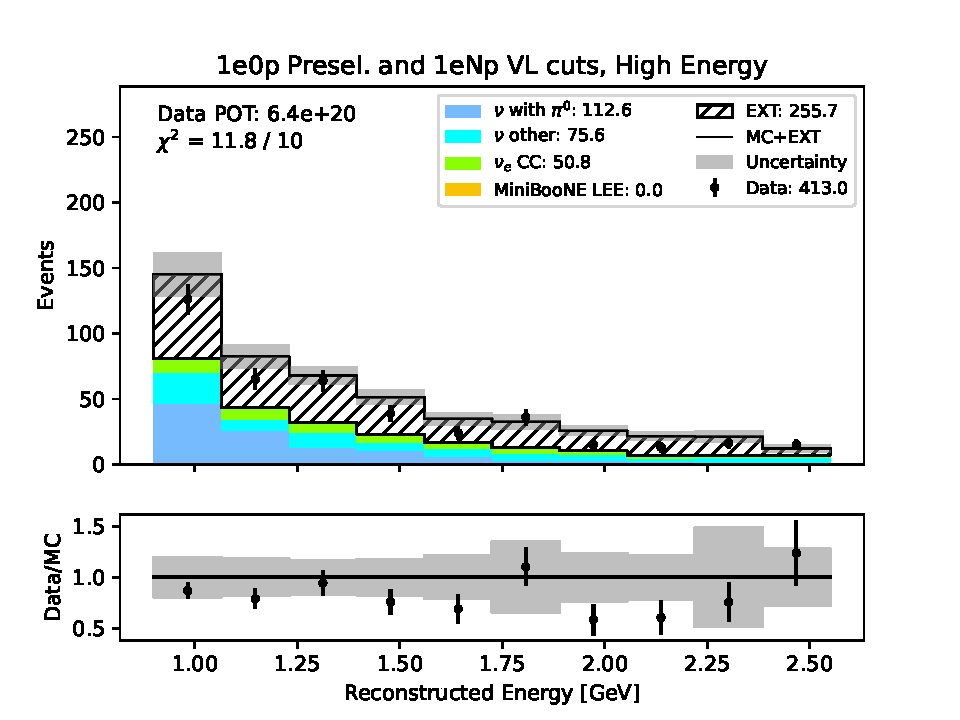
\includegraphics[width=\linewidth]{technote/Sidebands/Figures/FarSideband/far_sideband_reco_e_run123_ZP_ZP_HIGH_ENERGY.pdf}
    \caption{$\nu_e$ preselection, runs 1-3.}
    \end{subfigure}%
    \begin{subfigure}{0.5\linewidth}
    \includegraphics[width=\linewidth]{technote/Sidebands/Figures/FarSideband/far_sideband_reco_e_run123_ZP_ZPLOOSESEL_HIGH_ENERGY.pdf}
    \caption{1e0p loose selection, runs 1-3.}
    \end{subfigure}
    \begin{subfigure}{0.5\linewidth}
    \includegraphics[width=\linewidth]{technote/Sidebands/Figures/FarSideband/far_sideband_reco_e_run4b4c4d5_ZP_ZP_HIGH_ENERGY.pdf}
    \caption{$\nu_e$ preselection, runs 4-5}
    \end{subfigure}%
    \begin{subfigure}{0.5\linewidth}
    \includegraphics[width=\linewidth]{technote/Sidebands/Figures/FarSideband/far_sideband_reco_e_run4b4c4d5_ZP_ZPLOOSESEL_HIGH_ENERGY.pdf}
    \caption{1e0p loose selection, runs 4-5.}
    \end{subfigure}
    \begin{subfigure}{0.5\linewidth}
    \includegraphics[width=\linewidth]{technote/Sidebands/Figures/FarSideband/far_sideband_reco_e_run1234b4c4d5_ZP_ZP_HIGH_ENERGY.pdf}
    \caption{$\nu_e$ preselection., runs 1-5}
    \end{subfigure}%
    \begin{subfigure}{0.5\linewidth}
    \includegraphics[width=\linewidth]{technote/Sidebands/Figures/FarSideband/far_sideband_reco_e_run1234b4c4d5_ZP_ZPLOOSESEL_HIGH_ENERGY.pdf}
    \caption{1e0p loose selection, runs 1-5.}
    \end{subfigure}
    \caption{Reconstructed neutrino energy in the 1e0p high energy sideband.}
    \label{fig:HighEnergy1eNp_nonpi0_score}
\end{figure}

\begin{figure}[H]
    \centering
    \begin{subfigure}{0.5\linewidth}
    \includegraphics[width=\linewidth]{technote/Sidebands/Figures/FarSideband/far_sideband_bkg_score_run123_ZP_ZP_HIGH_ENERGY.pdf}
    \caption{$\nu_e$ preselection, runs 1-3.}
    \end{subfigure}%
    \begin{subfigure}{0.5\linewidth}
    \includegraphics[width=\linewidth]{technote/Sidebands/Figures/FarSideband/far_sideband_bkg_score_run123_ZP_ZPLOOSESEL_HIGH_ENERGY.pdf}
    \caption{1e0p loose selection, runs 1-3.}
    \end{subfigure}
    \begin{subfigure}{0.5\linewidth}
    \includegraphics[width=\linewidth]{technote/Sidebands/Figures/FarSideband/far_sideband_bkg_score_run4b4c4d5_ZP_ZP_HIGH_ENERGY.pdf}
    \caption{$\nu_e$ preselection, runs 4-5.}
    \end{subfigure}%
    \begin{subfigure}{0.5\linewidth}
    \includegraphics[width=\linewidth]{technote/Sidebands/Figures/FarSideband/far_sideband_bkg_score_run4b4c4d5_ZP_ZPLOOSESEL_HIGH_ENERGY.pdf}
    \caption{1e0p loose selection, runs 4-5.}
    \end{subfigure}
    \begin{subfigure}{0.5\linewidth}
    \includegraphics[width=\linewidth]{technote/Sidebands/Figures/FarSideband/far_sideband_bkg_score_run1234b4c4d5_ZP_ZP_HIGH_ENERGY.pdf}
    \caption{$\nu_e$ preselection, runs 1-5.}
    \end{subfigure}%
    \begin{subfigure}{0.5\linewidth}
    \includegraphics[width=\linewidth]{technote/Sidebands/Figures/FarSideband/far_sideband_bkg_score_run1234b4c4d5_ZP_ZPLOOSESEL_HIGH_ENERGY.pdf}
    \caption{1e0p loose selection, runs 1-5.}
    \end{subfigure}
    \caption{Reconstructed neutrino energy in the 1e0p high energy sideband.}
    \label{fig:HighEnergy1eNp_nonpi0_score}
\end{figure}

\begin{figure}[H]
    \centering
    \begin{subfigure}{0.33\linewidth}
        \includegraphics[width=\linewidth]{technote/Sidebands/Figures/FarSideband/far_sideband_dummy_run123_ZP_ZPBDT_HIGH_ENERGY.pdf}
    \caption{Runs 1-3.}
    \end{subfigure}%
    \begin{subfigure}{0.33\linewidth}
        \includegraphics[width=\linewidth]{technote/Sidebands/Figures/FarSideband/far_sideband_dummy_run4b4c4d5_ZP_ZPBDT_HIGH_ENERGY.pdf}
    \caption{Runs 4-5.}
    \end{subfigure}
    \begin{subfigure}{0.33\linewidth}
        \includegraphics[width=\linewidth]{technote/Sidebands/Figures/FarSideband/far_sideband_dummy_run1234b4c4d5_ZP_ZPBDT_HIGH_ENERGY.pdf}
    \caption{Runs 1-5.}
    \end{subfigure}
    \caption{Normalisation of data and MC simulation samples after application of the 1e0p BDT selection to the high energy sideband.}
\end{figure}
\subsection{Low BDT Score Sidebands}
\label{sec:LowBDTScoreSidebands}

The second set of sub-sidebands to inspect is obtained by selecting the low BDT scoring regions of the far sidebands. In the case of the 1eNp selection, this corresponds to the region with $\pi^0$ scores and non-$\pi^0$ scores both less than 0.1, while for the 1e0p selection, we require a background score less than 0.4. These sidebands are illustrated in Figure~\ref{fig:LowBDTSideband}.

\begin{figure}[H]
    \centering
    \begin{subfigure}{0.5\linewidth}
        \includegraphics[width=\linewidth]{technote/Sidebands/Figures/FarSideband/ZpLowBDTSideband.pdf}
        \caption{For the 1e0p selection.}
    \end{subfigure}%
    \begin{subfigure}{0.5\linewidth}
        \includegraphics[width=\linewidth]{technote/Sidebands/Figures/FarSideband/NpLowBDTSideband.pdf}
        \caption{For the 1eNp selection.}
    \end{subfigure}
    \caption{The low BDT score sidebands.}
    \label{fig:LowBDTSideband}
\end{figure}

\begin{figure}[H]
    \centering
    \begin{subfigure}{0.5\linewidth}
        \includegraphics[width=\linewidth]{technote/Sidebands/Figures/FarSideband/far_sideband_reco_e_run123_NP_NP_LOW_PID.pdf}
        \caption{$\nu_e$ preselection, runs 1-3.}
    \end{subfigure}%
    \begin{subfigure}{0.5\linewidth}
        \includegraphics[width=\linewidth]{technote/Sidebands/Figures/FarSideband/far_sideband_reco_e_run123_NP_NPL_LOW_PID.pdf}
        \caption{1eNp loose selection, runs 1-3.}
    \end{subfigure}
    \begin{subfigure}{0.5\linewidth}
        \includegraphics[width=\linewidth]{technote/Sidebands/Figures/FarSideband/far_sideband_reco_e_run4b4c4d5_NP_NP_LOW_PID.pdf}
        \caption{$\nu_e$ preselection, runs 4-5.}
    \end{subfigure}%
    \begin{subfigure}{0.5\linewidth}
        \includegraphics[width=\linewidth]{technote/Sidebands/Figures/FarSideband/far_sideband_reco_e_run4b4c4d5_NP_NPL_LOW_PID.pdf}
        \caption{1eNp loose selection, runs 4-5.}
    \end{subfigure}    
    \begin{subfigure}{0.5\linewidth}
        \includegraphics[width=\linewidth]{technote/Sidebands/Figures/FarSideband/far_sideband_reco_e_run1234b4c4d5_NP_NP_LOW_PID.pdf}
        \caption{$\nu_e$ preselection, runs 1-5.}
    \end{subfigure}%
    \begin{subfigure}{0.5\linewidth}
        \includegraphics[width=\linewidth]{technote/Sidebands/Figures/FarSideband/far_sideband_reco_e_run1234b4c4d5_NP_NPL_LOW_PID.pdf}
        \caption{1eNp loose selection, runs 1-5.}
    \end{subfigure}
    \caption{Reconstructed neutrino energy using the low BDT score sideband and the 1eNp selections.}
\end{figure}

\begin{figure}
    \centering
    \begin{subfigure}{0.33\linewidth}
        \includegraphics[width=\linewidth]{technote/Sidebands/Figures/FarSideband/far_sideband_reco_e_run1_NP_NPL_LOW_PID.pdf}
        \caption{run 1.}
    \end{subfigure}%
    \begin{subfigure}{0.33\linewidth}
        \includegraphics[width=\linewidth]{technote/Sidebands/Figures/FarSideband/far_sideband_reco_e_run2_NP_NPL_LOW_PID.pdf}
        \caption{run 2.}
    \end{subfigure}%
    \begin{subfigure}{0.33\linewidth}
        \includegraphics[width=\linewidth]{technote/Sidebands/Figures/FarSideband/far_sideband_reco_e_run3_NP_NPL_LOW_PID.pdf}
        \caption{run 3.}
    \end{subfigure}
    \begin{subfigure}{0.33\linewidth}
        \includegraphics[width=\linewidth]{technote/Sidebands/Figures/FarSideband/far_sideband_reco_e_run4b_NP_NPL_LOW_PID.pdf}
        \caption{run 4b.}
    \end{subfigure}%
    \begin{subfigure}{0.33\linewidth}
        \includegraphics[width=\linewidth]{technote/Sidebands/Figures/FarSideband/far_sideband_reco_e_run4c_NP_NPL_LOW_PID.pdf}
        \caption{run 4c.}
    \end{subfigure}
    \begin{subfigure}{0.33\linewidth}
        \includegraphics[width=\linewidth]{technote/Sidebands/Figures/FarSideband/far_sideband_reco_e_run4d_NP_NPL_LOW_PID.pdf}
        \caption{run 4d.}
    \end{subfigure}%
    \begin{subfigure}{0.33\linewidth}
        \includegraphics[width=\linewidth]{technote/Sidebands/Figures/FarSideband/far_sideband_reco_e_run5_NP_NPL_LOW_PID.pdf}
        \caption{run 5.}
    \end{subfigure}
\end{figure}

\begin{figure}[H]
    \centering
    \begin{subfigure}{0.5\linewidth}
        \includegraphics[width=\linewidth]{technote/Sidebands/Figures/FarSideband/far_sideband_reco_e_run123_ZP_ZP_LOW_PID.pdf}
        \caption{$\nu_e$ preselection, runs 1-3.}
    \end{subfigure}%
    \begin{subfigure}{0.5\linewidth}
        \includegraphics[width=\linewidth]{technote/Sidebands/Figures/FarSideband/far_sideband_reco_e_run123_ZP_ZPLOOSESEL_LOW_PID.pdf}
        \caption{1e0p loose selection, runs 1-3.}
    \end{subfigure}
    \begin{subfigure}{0.5\linewidth}
        \includegraphics[width=\linewidth]{technote/Sidebands/Figures/FarSideband/far_sideband_reco_e_run4b4c4d5_ZP_ZP_LOW_PID.pdf}
        \caption{$\nu_e$ preselection, runs 4-5.}
    \end{subfigure}%
    \begin{subfigure}{0.5\linewidth}
        \includegraphics[width=\linewidth]{technote/Sidebands/Figures/FarSideband/far_sideband_reco_e_run4b4c4d5_ZP_ZPLOOSESEL_LOW_PID.pdf}
        \caption{1e0p loose selection, runs 4-5.}
    \end{subfigure}    
    \begin{subfigure}{0.5\linewidth}
        \includegraphics[width=\linewidth]{technote/Sidebands/Figures/FarSideband/far_sideband_reco_e_run1234b4c4d5_ZP_ZP_LOW_PID.pdf}
        \caption{$\nu_e$ preselection, runs 1-5.}
    \end{subfigure}%
    \begin{subfigure}{0.5\linewidth}
        \includegraphics[width=\linewidth]{technote/Sidebands/Figures/FarSideband/far_sideband_reco_e_run1234b4c4d5_ZP_ZPLOOSESEL_LOW_PID.pdf}
        \caption{1e0p loose selection, runs 1-5.}
    \end{subfigure}
    \caption{Reconstructed neutrino energy using the low BDT score sideband and the 1e0p selections.}
\end{figure}

\subsection{Medium Energy Sidebands}
\label{sec:MediumEnergySidebands}

Moving closer to the signal region, we open the near sideband region, and select events with medium reconstructed energies. In the case of the 1eNp selection, this sideband contains events with reconstructed energies between 0.75 and 1.05~GeV, and for the 1e0p selection, events with reconstructed energies between 0.65 and 0.90~GeV. As with the other sidebands, we compare predictions to data for runs 1-3, runs 4-5 and runs 1-5, showing good data stability. These sidebands are illustrated in Figure~\ref{fig:MediumEnergySideband}.

\begin{figure}[H]
    \centering
    \begin{subfigure}{0.5\linewidth}
        \includegraphics[width=\linewidth]{technote/Sidebands/Figures/NearSideband/ZpMediumEnergySideband.pdf}
        \caption{For the 1e0p selection.}
    \end{subfigure}%
    \begin{subfigure}{0.5\linewidth}
        \includegraphics[width=\linewidth]{technote/Sidebands/Figures/NearSideband/NpMediumEnergySideband.pdf}
        \caption{For the 1eNp selection.}
    \end{subfigure}
    \caption{The medium energy sidebands.}
    \label{fig:MediumEnergySideband}
\end{figure}

\begin{figure}[H]
    \centering
    \begin{subfigure}{0.33\linewidth}
        \includegraphics[width=\linewidth]{technote/Sidebands/Figures/NearSideband/near_sideband_reco_e_run123_NP_NP_MEDIUM_ENERGY.pdf}
        \caption{$\nu_e$ preselection, runs 1-3.}
    \end{subfigure}%
    \begin{subfigure}{0.33\linewidth}
        \includegraphics[width=\linewidth]{technote/Sidebands/Figures/NearSideband/near_sideband_reco_e_run123_NP_NPL_MEDIUM_ENERGY.pdf}
        \caption{1eNp loose selection, runs 1-3.}
    \end{subfigure}%
    \begin{subfigure}{0.33\linewidth}
        \includegraphics[width=\linewidth]{technote/Sidebands/Figures/NearSideband/near_sideband_reco_e_run123_NP_NPBDT_MEDIUM_ENERGY.pdf}
        \caption{1eNp BDT selection, runs 1-3.}
    \end{subfigure}
    \begin{subfigure}{0.33\linewidth}
        \includegraphics[width=\linewidth]{technote/Sidebands/Figures/NearSideband/near_sideband_reco_e_run4b4c4d5_NP_NP_MEDIUM_ENERGY.pdf}
        \caption{$\nu_e$ preselection, runs 4-5.}
    \end{subfigure}%
    \begin{subfigure}{0.33\linewidth}
        \includegraphics[width=\linewidth]{technote/Sidebands/Figures/NearSideband/near_sideband_reco_e_run4b4c4d5_NP_NPL_MEDIUM_ENERGY.pdf}
        \caption{1eNp loose selection, runs 4-5.}
    \end{subfigure}%
    \begin{subfigure}{0.33\linewidth}
        \includegraphics[width=\linewidth]{technote/Sidebands/Figures/NearSideband/near_sideband_reco_e_run4b4c4d5_NP_NPBDT_MEDIUM_ENERGY.pdf}
        \caption{1eNp BDT selection, runs 4-5.}
    \end{subfigure}
    \begin{subfigure}{0.33\linewidth}
        \includegraphics[width=\linewidth]{technote/Sidebands/Figures/NearSideband/near_sideband_reco_e_run1234b4c4d5_NP_NP_MEDIUM_ENERGY.pdf}
        \caption{$\nu_e$ preselection, runs 1-5.}
    \end{subfigure}%
    \begin{subfigure}{0.33\linewidth}
        \includegraphics[width=\linewidth]{technote/Sidebands/Figures/NearSideband/near_sideband_reco_e_run1234b4c4d5_NP_NPL_MEDIUM_ENERGY.pdf}
        \caption{1eNp loose selection, runs 1-5.}
    \end{subfigure}%
    \begin{subfigure}{0.33\linewidth}
        \includegraphics[width=\linewidth]{technote/Sidebands/Figures/NearSideband/near_sideband_reco_e_run1234b4c4d5_NP_NPBDT_MEDIUM_ENERGY.pdf}
        \caption{1eNp BDT selection, runs 1-5.}
    \end{subfigure}
    \caption{Data and MC simulation comparisons in the 1eNp medium energy sideband.}
\end{figure}

\begin{figure}[H]
    \centering
    \begin{subfigure}{0.33\linewidth}
        \includegraphics[width=\linewidth]{technote/Sidebands/Figures/NearSideband/near_sideband_pi0_score_run123_NP_NP_MEDIUM_ENERGY.pdf}
        \caption{$\nu_e$ preselection, runs 1-3.}
    \end{subfigure}%
    \begin{subfigure}{0.33\linewidth}
        \includegraphics[width=\linewidth]{technote/Sidebands/Figures/NearSideband/near_sideband_pi0_score_run123_NP_NPL_MEDIUM_ENERGY.pdf}
        \caption{1eNp loose selection, runs 1-3.}
    \end{subfigure}%
    \begin{subfigure}{0.33\linewidth}
        \includegraphics[width=\linewidth]{technote/Sidebands/Figures/NearSideband/near_sideband_pi0_score_run123_NP_NPBDT_MEDIUM_ENERGY.pdf}
        \caption{1eNp BDT selection, runs 1-3.}
    \end{subfigure}
    \begin{subfigure}{0.33\linewidth}
        \includegraphics[width=\linewidth]{technote/Sidebands/Figures/NearSideband/near_sideband_pi0_score_run4b4c4d5_NP_NP_MEDIUM_ENERGY.pdf}
        \caption{$\nu_e$ preselection, runs 4-5.}
    \end{subfigure}%
    \begin{subfigure}{0.33\linewidth}
        \includegraphics[width=\linewidth]{technote/Sidebands/Figures/NearSideband/near_sideband_pi0_score_run4b4c4d5_NP_NPL_MEDIUM_ENERGY.pdf}
        \caption{1eNp loose selection, runs 4-5.}
    \end{subfigure}%
    \begin{subfigure}{0.33\linewidth}
        \includegraphics[width=\linewidth]{technote/Sidebands/Figures/NearSideband/near_sideband_pi0_score_run4b4c4d5_NP_NPBDT_MEDIUM_ENERGY.pdf}
        \caption{1eNp BDT selection, runs 4-5.}
    \end{subfigure}
    \begin{subfigure}{0.33\linewidth}
        \includegraphics[width=\linewidth]{technote/Sidebands/Figures/NearSideband/near_sideband_pi0_score_run1234b4c4d5_NP_NP_MEDIUM_ENERGY.pdf}
        \caption{$\nu_e$ preselection, runs 1-5.}
    \end{subfigure}%
    \begin{subfigure}{0.33\linewidth}
        \includegraphics[width=\linewidth]{technote/Sidebands/Figures/NearSideband/near_sideband_pi0_score_run1234b4c4d5_NP_NPL_MEDIUM_ENERGY.pdf}
        \caption{1eNp loose selection, runs 1-5.}
    \end{subfigure}%
    \begin{subfigure}{0.33\linewidth}
        \includegraphics[width=\linewidth]{technote/Sidebands/Figures/NearSideband/near_sideband_pi0_score_run1234b4c4d5_NP_NPBDT_MEDIUM_ENERGY.pdf}
        \caption{1eNp BDT selection, runs 1-5.}
    \end{subfigure}
    \caption{Data and MC simulation comparisons in the 1eNp medium energy sideband.}
\end{figure}

\begin{figure}[H]
    \centering
    \begin{subfigure}{0.33\linewidth}
        \includegraphics[width=\linewidth]{technote/Sidebands/Figures/NearSideband/near_sideband_nonpi0_score_run123_NP_NP_MEDIUM_ENERGY.pdf}
        \caption{$\nu_e$ preselection, runs 1-3.}
    \end{subfigure}%
    \begin{subfigure}{0.33\linewidth}
        \includegraphics[width=\linewidth]{technote/Sidebands/Figures/NearSideband/near_sideband_nonpi0_score_run123_NP_NPL_MEDIUM_ENERGY.pdf}
        \caption{1eNp loose selection, runs 1-3.}
    \end{subfigure}%
    \begin{subfigure}{0.33\linewidth}
        \includegraphics[width=\linewidth]{technote/Sidebands/Figures/NearSideband/near_sideband_nonpi0_score_run123_NP_NPBDT_MEDIUM_ENERGY.pdf}
        \caption{1eNp BDT selection, runs 1-3.}
    \end{subfigure}
    \begin{subfigure}{0.33\linewidth}
        \includegraphics[width=\linewidth]{technote/Sidebands/Figures/NearSideband/near_sideband_nonpi0_score_run4b4c4d5_NP_NP_MEDIUM_ENERGY.pdf}
        \caption{$\nu_e$ preselection, runs 4-5.}
    \end{subfigure}%
    \begin{subfigure}{0.33\linewidth}
        \includegraphics[width=\linewidth]{technote/Sidebands/Figures/NearSideband/near_sideband_nonpi0_score_run4b4c4d5_NP_NPL_MEDIUM_ENERGY.pdf}
        \caption{1eNp loose selection, runs 4-5.}
    \end{subfigure}%
    \begin{subfigure}{0.33\linewidth}
        \includegraphics[width=\linewidth]{technote/Sidebands/Figures/NearSideband/near_sideband_nonpi0_score_run4b4c4d5_NP_NPBDT_MEDIUM_ENERGY.pdf}
        \caption{1eNp BDT selection, runs 4-5.}
    \end{subfigure}    
    \begin{subfigure}{0.33\linewidth}
        \includegraphics[width=\linewidth]{technote/Sidebands/Figures/NearSideband/near_sideband_nonpi0_score_run1234b4c4d5_NP_NP_MEDIUM_ENERGY.pdf}
        \caption{$\nu_e$ preselection, runs 1-5.}
    \end{subfigure}%
    \begin{subfigure}{0.33\linewidth}
        \includegraphics[width=\linewidth]{technote/Sidebands/Figures/NearSideband/near_sideband_nonpi0_score_run1234b4c4d5_NP_NPL_MEDIUM_ENERGY.pdf}
        \caption{1eNp loose selection, runs 1-5.}
    \end{subfigure}%
    \begin{subfigure}{0.33\linewidth}
        \includegraphics[width=\linewidth]{technote/Sidebands/Figures/NearSideband/near_sideband_nonpi0_score_run1234b4c4d5_NP_NPBDT_MEDIUM_ENERGY.pdf}
        \caption{1eNp BDT selection, runs 1-5.}
    \end{subfigure}
    \caption{Data and MC simulation comparisons in the 1eNp medium energy sideband.}
\end{figure}

\begin{figure}[H]
    \centering
    \begin{subfigure}{0.5\linewidth}
        \includegraphics[width=\linewidth]{technote/Sidebands/Figures/NearSideband/near_sideband_reco_e_run123_ZP_ZP_MEDIUM_ENERGY.pdf}
        \caption{$\nu_e$ preselection, runs 1-3.}
    \end{subfigure}%
    \begin{subfigure}{0.5\linewidth}
        \includegraphics[width=\linewidth]{technote/Sidebands/Figures/NearSideband/near_sideband_reco_e_run123_ZP_ZPLOOSESEL_MEDIUM_ENERGY.pdf}
        \caption{Loose selection, runs 1-3.}
    \end{subfigure}
    \begin{subfigure}{0.5\linewidth}
        \includegraphics[width=\linewidth]{technote/Sidebands/Figures/NearSideband/near_sideband_reco_e_run4b4c4d5_ZP_ZP_MEDIUM_ENERGY.pdf}
        \caption{$\nu_e$ preselection, runs 4-5.}
    \end{subfigure}%
    \begin{subfigure}{0.5\linewidth}
        \includegraphics[width=\linewidth]{technote/Sidebands/Figures/NearSideband/near_sideband_reco_e_run4b4c4d5_ZP_ZPLOOSESEL_MEDIUM_ENERGY.pdf}
        \caption{Loose selection, runs 4-5.}
    \end{subfigure}
    \begin{subfigure}{0.5\linewidth}
        \includegraphics[width=\linewidth]{technote/Sidebands/Figures/NearSideband/near_sideband_reco_e_run1234b4c4d5_ZP_ZP_MEDIUM_ENERGY.pdf}
        \caption{$\nu_e$ preselection, runs 1-5.}
    \end{subfigure}%
    \begin{subfigure}{0.5\linewidth}
        \includegraphics[width=\linewidth]{technote/Sidebands/Figures/NearSideband/near_sideband_reco_e_run1234b4c4d5_ZP_ZPLOOSESEL_MEDIUM_ENERGY.pdf}
        \caption{Loose selection, runs 1-5.}
    \end{subfigure}
    \caption{Data and MC simulation comparisons in the 1e0p medium energy sideband.}
\end{figure}

\begin{figure}[H]
    \centering
    \begin{subfigure}{0.5\linewidth}
        \includegraphics[width=\linewidth]{technote/Sidebands/Figures/NearSideband/near_sideband_bkg_score_run123_ZP_ZP_MEDIUM_ENERGY.pdf}
        \caption{$\nu_e$ preselection, runs 1-3.}
    \end{subfigure}%
    \begin{subfigure}{0.5\linewidth}
        \includegraphics[width=\linewidth]{technote/Sidebands/Figures/NearSideband/near_sideband_bkg_score_run123_ZP_ZPLOOSESEL_MEDIUM_ENERGY.pdf}
        \caption{Loose selection, runs 1-3.}
    \end{subfigure}
    \begin{subfigure}{0.5\linewidth}
        \includegraphics[width=\linewidth]{technote/Sidebands/Figures/NearSideband/near_sideband_bkg_score_run4b4c4d5_ZP_ZP_MEDIUM_ENERGY.pdf}
        \caption{$\nu_e$ preselection, runs 4-5.}
    \end{subfigure}%
    \begin{subfigure}{0.5\linewidth}
        \includegraphics[width=\linewidth]{technote/Sidebands/Figures/NearSideband/near_sideband_bkg_score_run4b4c4d5_ZP_ZPLOOSESEL_MEDIUM_ENERGY.pdf}
        \caption{Loose selection, runs 4-5.}
    \end{subfigure}
    \begin{subfigure}{0.5\linewidth}
        \includegraphics[width=\linewidth]{technote/Sidebands/Figures/NearSideband/near_sideband_bkg_score_run1234b4c4d5_ZP_ZP_MEDIUM_ENERGY.pdf}
        \caption{$\nu_e$ preselection, runs 1-5.}
    \end{subfigure}%
    \begin{subfigure}{0.5\linewidth}
        \includegraphics[width=\linewidth]{technote/Sidebands/Figures/NearSideband/near_sideband_bkg_score_run1234b4c4d5_ZP_ZPLOOSESEL_MEDIUM_ENERGY.pdf}
        \caption{Loose selection, runs 1-5.}
    \end{subfigure}
    \caption{Data and MC simulation comparisons in the 1e0p medium energy sideband.}
\end{figure}


\subsection{Medium BDT Score Sidebands}
\label{sec:MediumBDTScoreSidebands}

We can inspect the full energy spectrum whilst keeping the signal region blind by applying cuts to the BDT scores. The medium BDT score sidebands are constructed by selecting events from the near sidebands with background scores between 0.4 and 0.72 in the case of the 1e0p selection. When applying the 1eNp selection, we only include events that have both $0.1<$ $\pi^0$ score $< 0.67$, and $0.1<$ non-$\pi^0$ score $< 0.70$. 

\begin{figure}[H]
    \centering
    \begin{subfigure}{0.5\linewidth}
        \includegraphics[width=\linewidth]{technote/Sidebands/Figures/NearSideband/ZpMediumBDTSideband.pdf}
        \caption{For the 1e0p selection.}
    \end{subfigure}%
    \begin{subfigure}{0.5\linewidth}
        \includegraphics[width=\linewidth]{technote/Sidebands/Figures/NearSideband/NpMediumBDTSideband.pdf}
        \caption{For the 1eNp selection.}
    \end{subfigure}
    \caption{The BDT score sidebands.}
    \label{fig:MediumBDTSideband}
\end{figure}

\begin{figure}[H]
    \centering
    \begin{subfigure}{0.5\linewidth}
        \includegraphics[width=\linewidth]{technote/Sidebands/Figures/NearSideband/near_sideband_reco_e_run123_NP_NP_MEDIUM_PID.pdf}
        \caption{$\nu_e$ preselection, runs 1-3.}
    \end{subfigure}%
    \begin{subfigure}{0.5\linewidth}
        \includegraphics[width=\linewidth]{technote/Sidebands/Figures/NearSideband/near_sideband_reco_e_run123_NP_NPL_MEDIUM_PID.pdf}
        \caption{1eNp loose selection, runs 1-3.}
    \end{subfigure}
    \begin{subfigure}{0.5\linewidth}
        \includegraphics[width=\linewidth]{technote/Sidebands/Figures/NearSideband/near_sideband_reco_e_run4b4c4d5_NP_NP_MEDIUM_PID.pdf}
        \caption{$\nu_e$ preselection, runs 4-5.}
    \end{subfigure}%
    \begin{subfigure}{0.5\linewidth}
        \includegraphics[width=\linewidth]{technote/Sidebands/Figures/NearSideband/near_sideband_reco_e_run4b4c4d5_NP_NPL_MEDIUM_PID.pdf}
        \caption{1eNp loose selection, runs 4-5.}
    \end{subfigure}    
    \begin{subfigure}{0.5\linewidth}
        \includegraphics[width=\linewidth]{technote/Sidebands/Figures/NearSideband/near_sideband_reco_e_run1234b4c4d5_NP_NP_MEDIUM_PID.pdf}
        \caption{$\nu_e$ preselection, runs 1-5.}
    \end{subfigure}%
    \begin{subfigure}{0.5\linewidth}
        \includegraphics[width=\linewidth]{technote/Sidebands/Figures/NearSideband/near_sideband_reco_e_run1234b4c4d5_NP_NPL_MEDIUM_PID.pdf}
        \caption{1eNp loose selection, runs 1-5.}
    \end{subfigure}
    \caption{Data and MC simulation comparisons in the 1eNp medium BDT score sideband.}
\end{figure}

\begin{figure}[H]
    \centering
    \begin{subfigure}{0.5\linewidth}
        \includegraphics[width=\linewidth]{technote/Sidebands/Figures/NearSideband/near_sideband_pi0_score_run123_NP_NP_MEDIUM_PID.pdf}
        \caption{$\nu_e$ preselection, runs 1-3.}
    \end{subfigure}%
    \begin{subfigure}{0.5\linewidth}
        \includegraphics[width=\linewidth]{technote/Sidebands/Figures/NearSideband/near_sideband_pi0_score_run123_NP_NPL_MEDIUM_PID.pdf}
        \caption{1eNp loose selection, runs 1-3.}
    \end{subfigure}
    \begin{subfigure}{0.5\linewidth}
        \includegraphics[width=\linewidth]{technote/Sidebands/Figures/NearSideband/near_sideband_pi0_score_run4b4c4d5_NP_NP_MEDIUM_PID.pdf}
        \caption{$\nu_e$ preselection, runs 4-5.}
    \end{subfigure}%
    \begin{subfigure}{0.5\linewidth}
        \includegraphics[width=\linewidth]{technote/Sidebands/Figures/NearSideband/near_sideband_pi0_score_run4b4c4d5_NP_NPL_MEDIUM_PID.pdf}
        \caption{1eNp loose selection, runs 4-5.}
    \end{subfigure}    
    \begin{subfigure}{0.5\linewidth}
        \includegraphics[width=\linewidth]{technote/Sidebands/Figures/NearSideband/near_sideband_pi0_score_run1234b4c4d5_NP_NP_MEDIUM_PID.pdf}
        \caption{$\nu_e$ preselection, runs 1-5.}
    \end{subfigure}%
    \begin{subfigure}{0.5\linewidth}
        \includegraphics[width=\linewidth]{technote/Sidebands/Figures/NearSideband/near_sideband_pi0_score_run1234b4c4d5_NP_NPL_MEDIUM_PID.pdf}
        \caption{1eNp loose selection, runs 1-5.}
    \end{subfigure}
    \caption{Data and MC simulation comparisons in the 1eNp medium BDT score sideband.}
\end{figure}

\begin{figure}[H]
    \centering
    \begin{subfigure}{0.5\linewidth}
        \includegraphics[width=\linewidth]{technote/Sidebands/Figures/NearSideband/near_sideband_nonpi0_score_run123_NP_NP_MEDIUM_PID.pdf}
        \caption{$\nu_e$ preselection, runs 1-3.}
    \end{subfigure}%
    \begin{subfigure}{0.5\linewidth}
        \includegraphics[width=\linewidth]{technote/Sidebands/Figures/NearSideband/near_sideband_nonpi0_score_run123_NP_NPL_MEDIUM_PID.pdf}
        \caption{1eNp loose selection, runs 1-3.}
    \end{subfigure}
    \begin{subfigure}{0.5\linewidth}
        \includegraphics[width=\linewidth]{technote/Sidebands/Figures/NearSideband/near_sideband_nonpi0_score_run4b4c4d5_NP_NP_MEDIUM_PID.pdf}
        \caption{$\nu_e$ preselection, runs 4-5.}
    \end{subfigure}%
    \begin{subfigure}{0.5\linewidth}
        \includegraphics[width=\linewidth]{technote/Sidebands/Figures/NearSideband/near_sideband_nonpi0_score_run4b4c4d5_NP_NPL_MEDIUM_PID.pdf}
        \caption{1eNp loose selection, runs 4-5.}
    \end{subfigure}    
    \begin{subfigure}{0.5\linewidth}
        \includegraphics[width=\linewidth]{technote/Sidebands/Figures/NearSideband/near_sideband_nonpi0_score_run1234b4c4d5_NP_NP_MEDIUM_PID.pdf}
        \caption{$\nu_e$ preselection, runs 1-5.}
    \end{subfigure}%
    \begin{subfigure}{0.5\linewidth}
        \includegraphics[width=\linewidth]{technote/Sidebands/Figures/NearSideband/near_sideband_nonpi0_score_run1234b4c4d5_NP_NPL_MEDIUM_PID.pdf}
        \caption{1eNp loose selection, runs 1-5.}
    \end{subfigure}
    \caption{Data and MC simulation comparisons in the 1e0p medium BDT score sideband.}
\end{figure}

\begin{figure}[H]
    \centering
    \begin{subfigure}{0.5\linewidth}
        \includegraphics[width=\linewidth]{technote/Sidebands/Figures/NearSideband/near_sideband_reco_e_run123_ZP_ZP_MEDIUM_PID.pdf}
        \caption{$\nu_e$ preselection, runs 1-3.}
    \end{subfigure}%
    \begin{subfigure}{0.5\linewidth}
        \includegraphics[width=\linewidth]{technote/Sidebands/Figures/NearSideband/near_sideband_reco_e_run123_ZP_ZPLOOSESEL_MEDIUM_PID.pdf}
        \caption{1e0p loose selection, runs 1-3.}
    \end{subfigure}
    \begin{subfigure}{0.5\linewidth}
        \includegraphics[width=\linewidth]{technote/Sidebands/Figures/NearSideband/near_sideband_reco_e_run4b4c4d5_ZP_ZP_MEDIUM_PID.pdf}
        \caption{$\nu_e$ preselection, runs 4-5.}
    \end{subfigure}%
    \begin{subfigure}{0.5\linewidth}
        \includegraphics[width=\linewidth]{technote/Sidebands/Figures/NearSideband/near_sideband_reco_e_run4b4c4d5_ZP_ZPLOOSESEL_MEDIUM_PID.pdf}
        \caption{1e0p loose selection, runs 4-5.}
    \end{subfigure}    
    \begin{subfigure}{0.5\linewidth}
        \includegraphics[width=\linewidth]{technote/Sidebands/Figures/NearSideband/near_sideband_reco_e_run1234b4c4d5_ZP_ZP_MEDIUM_PID.pdf}
        \caption{$\nu_e$ preselection, runs 1-5.}
    \end{subfigure}%
    \begin{subfigure}{0.5\linewidth}
        \includegraphics[width=\linewidth]{technote/Sidebands/Figures/NearSideband/near_sideband_reco_e_run1234b4c4d5_ZP_ZPLOOSESEL_MEDIUM_PID.pdf}
        \caption{1e0p loose selection, runs 1-5.}
    \end{subfigure}
    \caption{Data and MC simulation comparisons in the 1e0p medium BDT score sideband.}
\end{figure}

\begin{figure}[H]
    \centering
    \begin{subfigure}{0.5\linewidth}
        \includegraphics[width=\linewidth]{technote/Sidebands/Figures/NearSideband/near_sideband_bkg_score_run123_ZP_ZP_MEDIUM_PID.pdf}
        \caption{$\nu_e$ preselection, runs 1-3.}
    \end{subfigure}%
    \begin{subfigure}{0.5\linewidth}
        \includegraphics[width=\linewidth]{technote/Sidebands/Figures/NearSideband/near_sideband_bkg_score_run123_ZP_ZPLOOSESEL_MEDIUM_PID.pdf}
        \caption{1e0p loose selection, runs 1-3.}
    \end{subfigure}
    \begin{subfigure}{0.5\linewidth}
        \includegraphics[width=\linewidth]{technote/Sidebands/Figures/NearSideband/near_sideband_bkg_score_run4b4c4d5_ZP_ZPLOOSESEL_MEDIUM_PID.pdf}
        \caption{$\nu_e$ preselection, runs 4-5.}
    \end{subfigure}%
    \begin{subfigure}{0.5\linewidth}
        \includegraphics[width=\linewidth]{technote/Sidebands/Figures/NearSideband/near_sideband_bkg_score_run4b4c4d5_ZP_ZPLOOSESEL_MEDIUM_PID.pdf}
        \caption{1e0p loose selection, runs 4-5.}
    \end{subfigure}    
    \begin{subfigure}{0.5\linewidth}
        \includegraphics[width=\linewidth]{technote/Sidebands/Figures/NearSideband/near_sideband_bkg_score_run1234b4c4d5_ZP_ZPLOOSESEL_MEDIUM_PID.pdf}
        \caption{$\nu_e$ preselection, runs 1-5.}
    \end{subfigure}%
    \begin{subfigure}{0.5\linewidth}
        \includegraphics[width=\linewidth]{technote/Sidebands/Figures/NearSideband/near_sideband_bkg_score_run1234b4c4d5_ZP_ZPLOOSESEL_MEDIUM_PID.pdf}
        \caption{1e0p loose selection, runs 1-5.}
    \end{subfigure}
    \caption{Data and MC simulation comparisons in the 1e0p medium BDT score sideband.}
\end{figure}
%\input{technote/Sidebands/ShowerEnergy}